\documentclass[a4paper,utf8]{article}
\usepackage[heading,fancyhdr]{ctex}
\usepackage{amsmath,amssymb,geometry,lastpage,ulem}
\usepackage{array,tabularx,tabulary,mhchem,xspace}
\usepackage{floatrow,subfig,multirow,bigstrut}
\usepackage{siunitx,booktabs,longtable,graphicx,xfrac,nameref}
\lineskiplimit=1pt
\lineskip=3pt
\geometry{
    top=25.4mm, 
    left=25mm, 
    right=25mm, 
    bottom=25mm,
    headsep=5.9mm,
}
\ctexset{
    section = {format+=\raggedright}
}
\newcommand{\fgref}[1]{图~\ref{#1}\xspace}
\newcommand{\seqref}[1]{式~(\ref{#1})}
\newcommand{\expinfo}[7][无]{
    {\zihao{-3}\bfseries\songti
    实验名称:\uline{\hfill\mbox{#2}\hfill} \\[2.9mm]
    学\quad 号:\uline{\makebox[25mm]{#3}}\hfill
    姓\quad 名:\uline{\makebox[25mm]{#4}}\hfill
    班\quad 级:\uline{\makebox[25mm]{#5}} \\[2.9mm]
    合作者:\uline{\makebox[25mm]{#1}} \hfill
    桌\quad 号:\uline{\makebox[25mm]{#6}}\hfill\makebox[25mm+4em]{}\\[2.9mm]
    实验日期:\uline{\makebox[30mm]{#7}}\hfill\mbox{} \\[58.7mm]
    }
}
\newcommand{\pointingbox}{
    {\zihao{4}\bfseries\songti%
    实验考核\\[3mm]
    \extrarowheight=3mm
    \begin{tabularx}{150mm}{|X|X|X|X|X|}\hline
        \hfil 项目 \hfil  & \hfil 实验预习 \hfil & \hfil 实验过程 \hfil & \hfil 分析与讨论 \hfil & \hfil 总评 \hfil \\[3mm] \hline
        \hfil 评价 \hfil &  &  &  &  \\[3mm] \hline
    \end{tabularx}
    }
}
\newcommand{\derivative}[2]{\frac{\mathrm{d} #1}{\mathrm{d} #2}}
\newcommand{\thinking}[2]{\textbf{#1}\\
答:\begin{minipage}[t]{0.85\textwidth}
    #2
\end{minipage}}
\pagestyle{fancy}
\fancyhf{} \fancyhead[C]{电路基础实验} \fancyfoot[C]{\thepage~/~\pageref{LastPage}}
\newcounter{Rownumber}
\newcommand*{\Rown}{\stepcounter{Rownumber}\theRownumber}
\newcommand*{\resetRown}{\setcounter{Rownumber}{0}}
\newcommand{\qrange}[3]{\qtyrange[range-phrase = \text{$\sim$},range-units =single]{#1}{#2}{#3}}
\floatsetup[table]{capposition=top}
\newcolumntype{C}{>{\hfil}X<{\hfil}}
\renewcommand{\Nameref}[1]{\textbf{\ref{#1}~\nameref{#1}}} %导入导言
\ctikzset{
    resistors/scale=0.7,
    diodes/scale=0.6}
\begin{document}
\begin{center}
    {\mbox{}\\[7em]\zihao{2}\bfseries\songti%
    电路基础实验报告}\\[34mm]
    \expinfo[王慷]{常用电信号的观察与测量}{22301056}{王俊杰}{22 材物}{27}{2024.5.28}
\end{center}
\newpage
\section{实验目的}
\begin{enumerate}
    \item 了解信号发生器与示波器的基本功能和使用方法。
    \item 掌握常用电信号的参数意义与测量方法。
\end{enumerate}

\section{实验原理}%简单描述,含必要的公式和附图;
\subsection{正弦信号}
一个正弦信号可表示为 $x(t) = A\sin(\omega t+\varphi)=A\cos(\omega t+\varphi-\pi/2)$ 。式中,$A$ 为振幅,$\omega$ 为角频率(弧度/秒),$\varphi$ 为初始相角(弧度),这三个参量称为正弦信号的三要素。除了这三个要素,正弦信号还有周期 $T$ 和频率 $f$ 两个参数,他们之间的关系为:$T=2\pi/\omega=1/f$。\par
常用表示幅度的还有峰峰值($V_\text{pp}$)和有效值($V_\text{rms}$)。$V_\text{pp}$ 与 $V_\text{rms}$ 之间的换算关系是 $V_\text{pp}=2\sqrt{2} V_\text{rms}$,万用表交流电压档测量的结果就是电压的有效值。
\subsection{方波信号}
电流或电压的波形为矩形的信号为矩形波信号,高电平在一个波形周期内占有的时间比值称为占空比,占空比为 50\% 的矩形波称之为方波。

\section{实验仪表}
    RIGOL DM3058 万用表、RIGOL MSO2202A 示波器、电路分析实验箱、导线若干。
\section{实验内容与结果}
\subsection{测量正弦信号参数}
设置信号发生器通道 1 输出 $V_\text{pp}=\SI{5}{\V}$,$f=\SI{1}{\kilo\Hz}$,偏移为 \SI{0}{\V} 的正弦波,分别用万用表 AC V(交流电压)档和 DC V(直流电压)档测量并记录正弦信号的交流电压值和直流电压值。将信号发生器输出与示波器通道1连接,调整示波器的水平、垂直和触发等参数,使示波器屏幕上显示 2-3 个完整信号周期,信号幅度占屏幕高度的四分之三左右,波形稳定不移动,波形如图 \ref{fig:8.1} 所示。根据附表 8-1 的要求,分别使用数格子、光标测量(设置光标模式为手动,显示模式为X-Y)、示波器自动测量功能测量信号的峰峰值、有效值、周期和频率等参数并记录。记录结果如表 \ref{tab:8.1} 所示。
\begin{table}[!ht]
    \caption{通道 1 测量偏移为 0 的正弦波参数\label{tab:8.1}}
    \begin{tabularx}{\textwidth}{|*{5}{X|}} \hline
        \hfil 信号发生器 & \multicolumn{4}{c|}{\multirow{2}*{通道 1 $V_\text{pp}=\SI{5}{\V}$,$f=\SI{1}{\kilo\Hz}$,偏移为 \SI{0}{\V} 的正弦波}} \\
        \hfil 设置 & \multicolumn{4}{c|}{} \\ \hline
        & 万用表测量 & 数格子测量 & 光标测量 & 自动测量 \\ \cline{2-5}
        测量方法与结果 & AC V = \SI{1.759}{\V} & 峰峰值 = \SI{5}{\V} & 峰峰值 = \SI{5.12}{\V} & 有效值 = \SI{1.818}{\V} \\
        & DC V = \SI{0}{\V} & 周期 = \SI{1}{\ms} & 周期 = \SI{1}{\ms} & 频率 = \SI{1000}{\Hz} \\ \hline
    \end{tabularx}
\end{table}
\begin{figure}[!ht]
    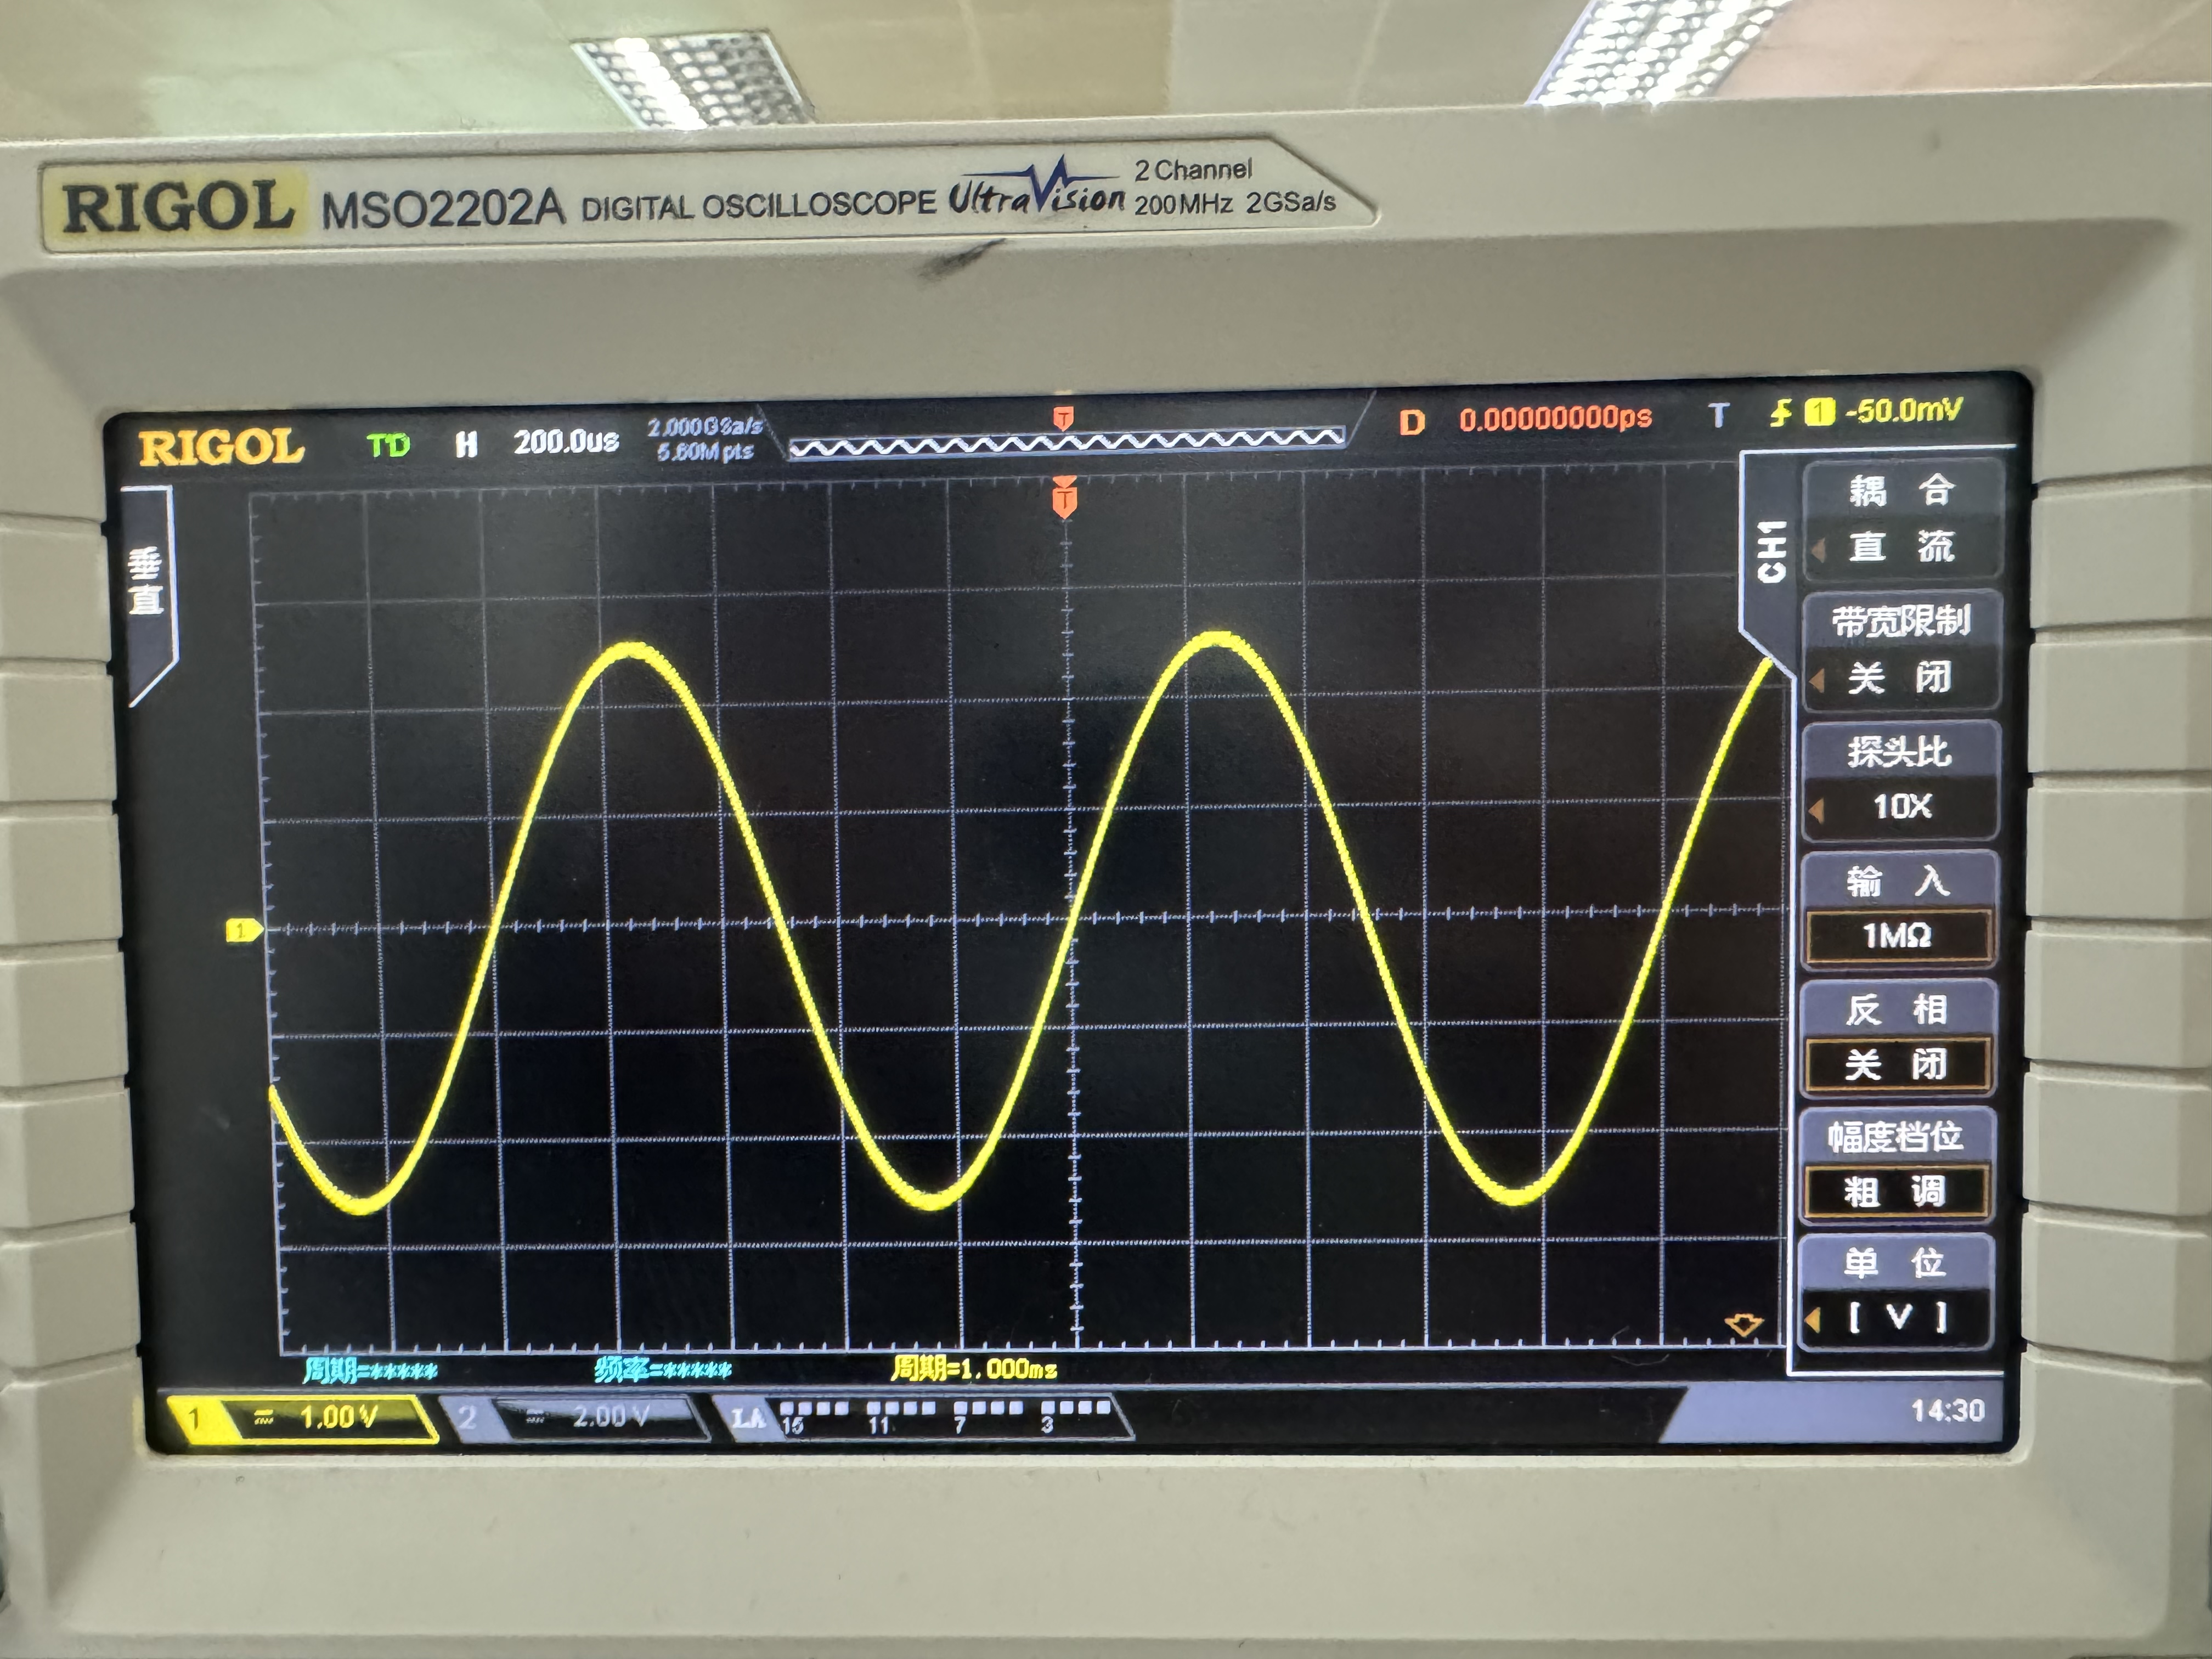
\includegraphics[width=0.4\textwidth]{8_1.jpg}
    \caption{通道 1 测量偏移为 \SI{0}{\V} 的正弦波\label{fig:8.1}}
\end{figure}

\subsection{观察测量有直流偏移的正弦信号和不同耦合方式下的波形\label{sss:ouhe}}
断开信号发生器通道 1 与示波器的连接,设置函数信号发生器通道 2 输出 $V_\text{pp}=\SI{5}{\V}$,$f=\SI{1}{\kilo\Hz}$,偏移为 \SI{1}{\V} 的正弦波,用万用表 AC V(交流电压)档 DC V(直流电压)档测量并记录正弦信号的交流电压值和直流电压值 (测量直流电压时,将万用表的量程设置为 \SI{20}{\V})。将信号发生器输出与示波器通道 2 连接,设置示波器通道 2 为直流耦合,调整示波器的水平、垂直和触发等参数,使示波器屏幕上显示 2-3 个完整信号周期,信号幅度占屏幕高度的四分之三左右,波形稳定不移动,波形如图 \ref{fig:8.2a} 所示,用示波器自动测量功能测量信号的峰峰值和有效值。然后将示波器通道 2 设置为交流耦合,观察波形有什么变化,波形如图 \ref{fig:8.2b} 所示,再次用示波器自动测量功能测量信号的峰峰值和有效值。数据记录到表 \ref{tab:8.2}。
\begin{table}[!ht]
    \caption{通道 2测量偏移为 \SI{1}{\V} 的正弦波参数\label{tab:8.2}}
    \begin{tabularx}{\textwidth}{|*{4}{X|}} \hline
        \hfil 信号发生器 & \multicolumn{3}{c|}{\multirow{2}*{通道 1 $V_\text{pp}=\SI{5}{\V}$,$f=\SI{1}{\kilo\Hz}$,偏移为 \SI{0}{\V} 的正弦波}} \\
        \hfil 设置 & \multicolumn{3}{c|}{} \\ \hline
        \multirow{4}*{测量方法与结果} & \multirow{2}*{万用表测量} & \multicolumn{2}{c|}{示波器自动测量} \\ \cline{3-4}
        & & 直流耦合 & 交流耦合 \\ \cline{2-4}
        & AC V = \SI{1.760}{\V} & 峰峰值 = \SI{5.160}{\V} & 峰峰值 = \SI{5.200}{\V} \\
        & DC V = \SI{117}{\mV} & 有效值 = \SI{2.102}{\V} & 有效值 = \SI{1.847}{\V} \\ \hline
    \end{tabularx}
\end{table}
\begin{figure}[!ht]
    \subfloat[直流耦合\label{fig:8.2a}]{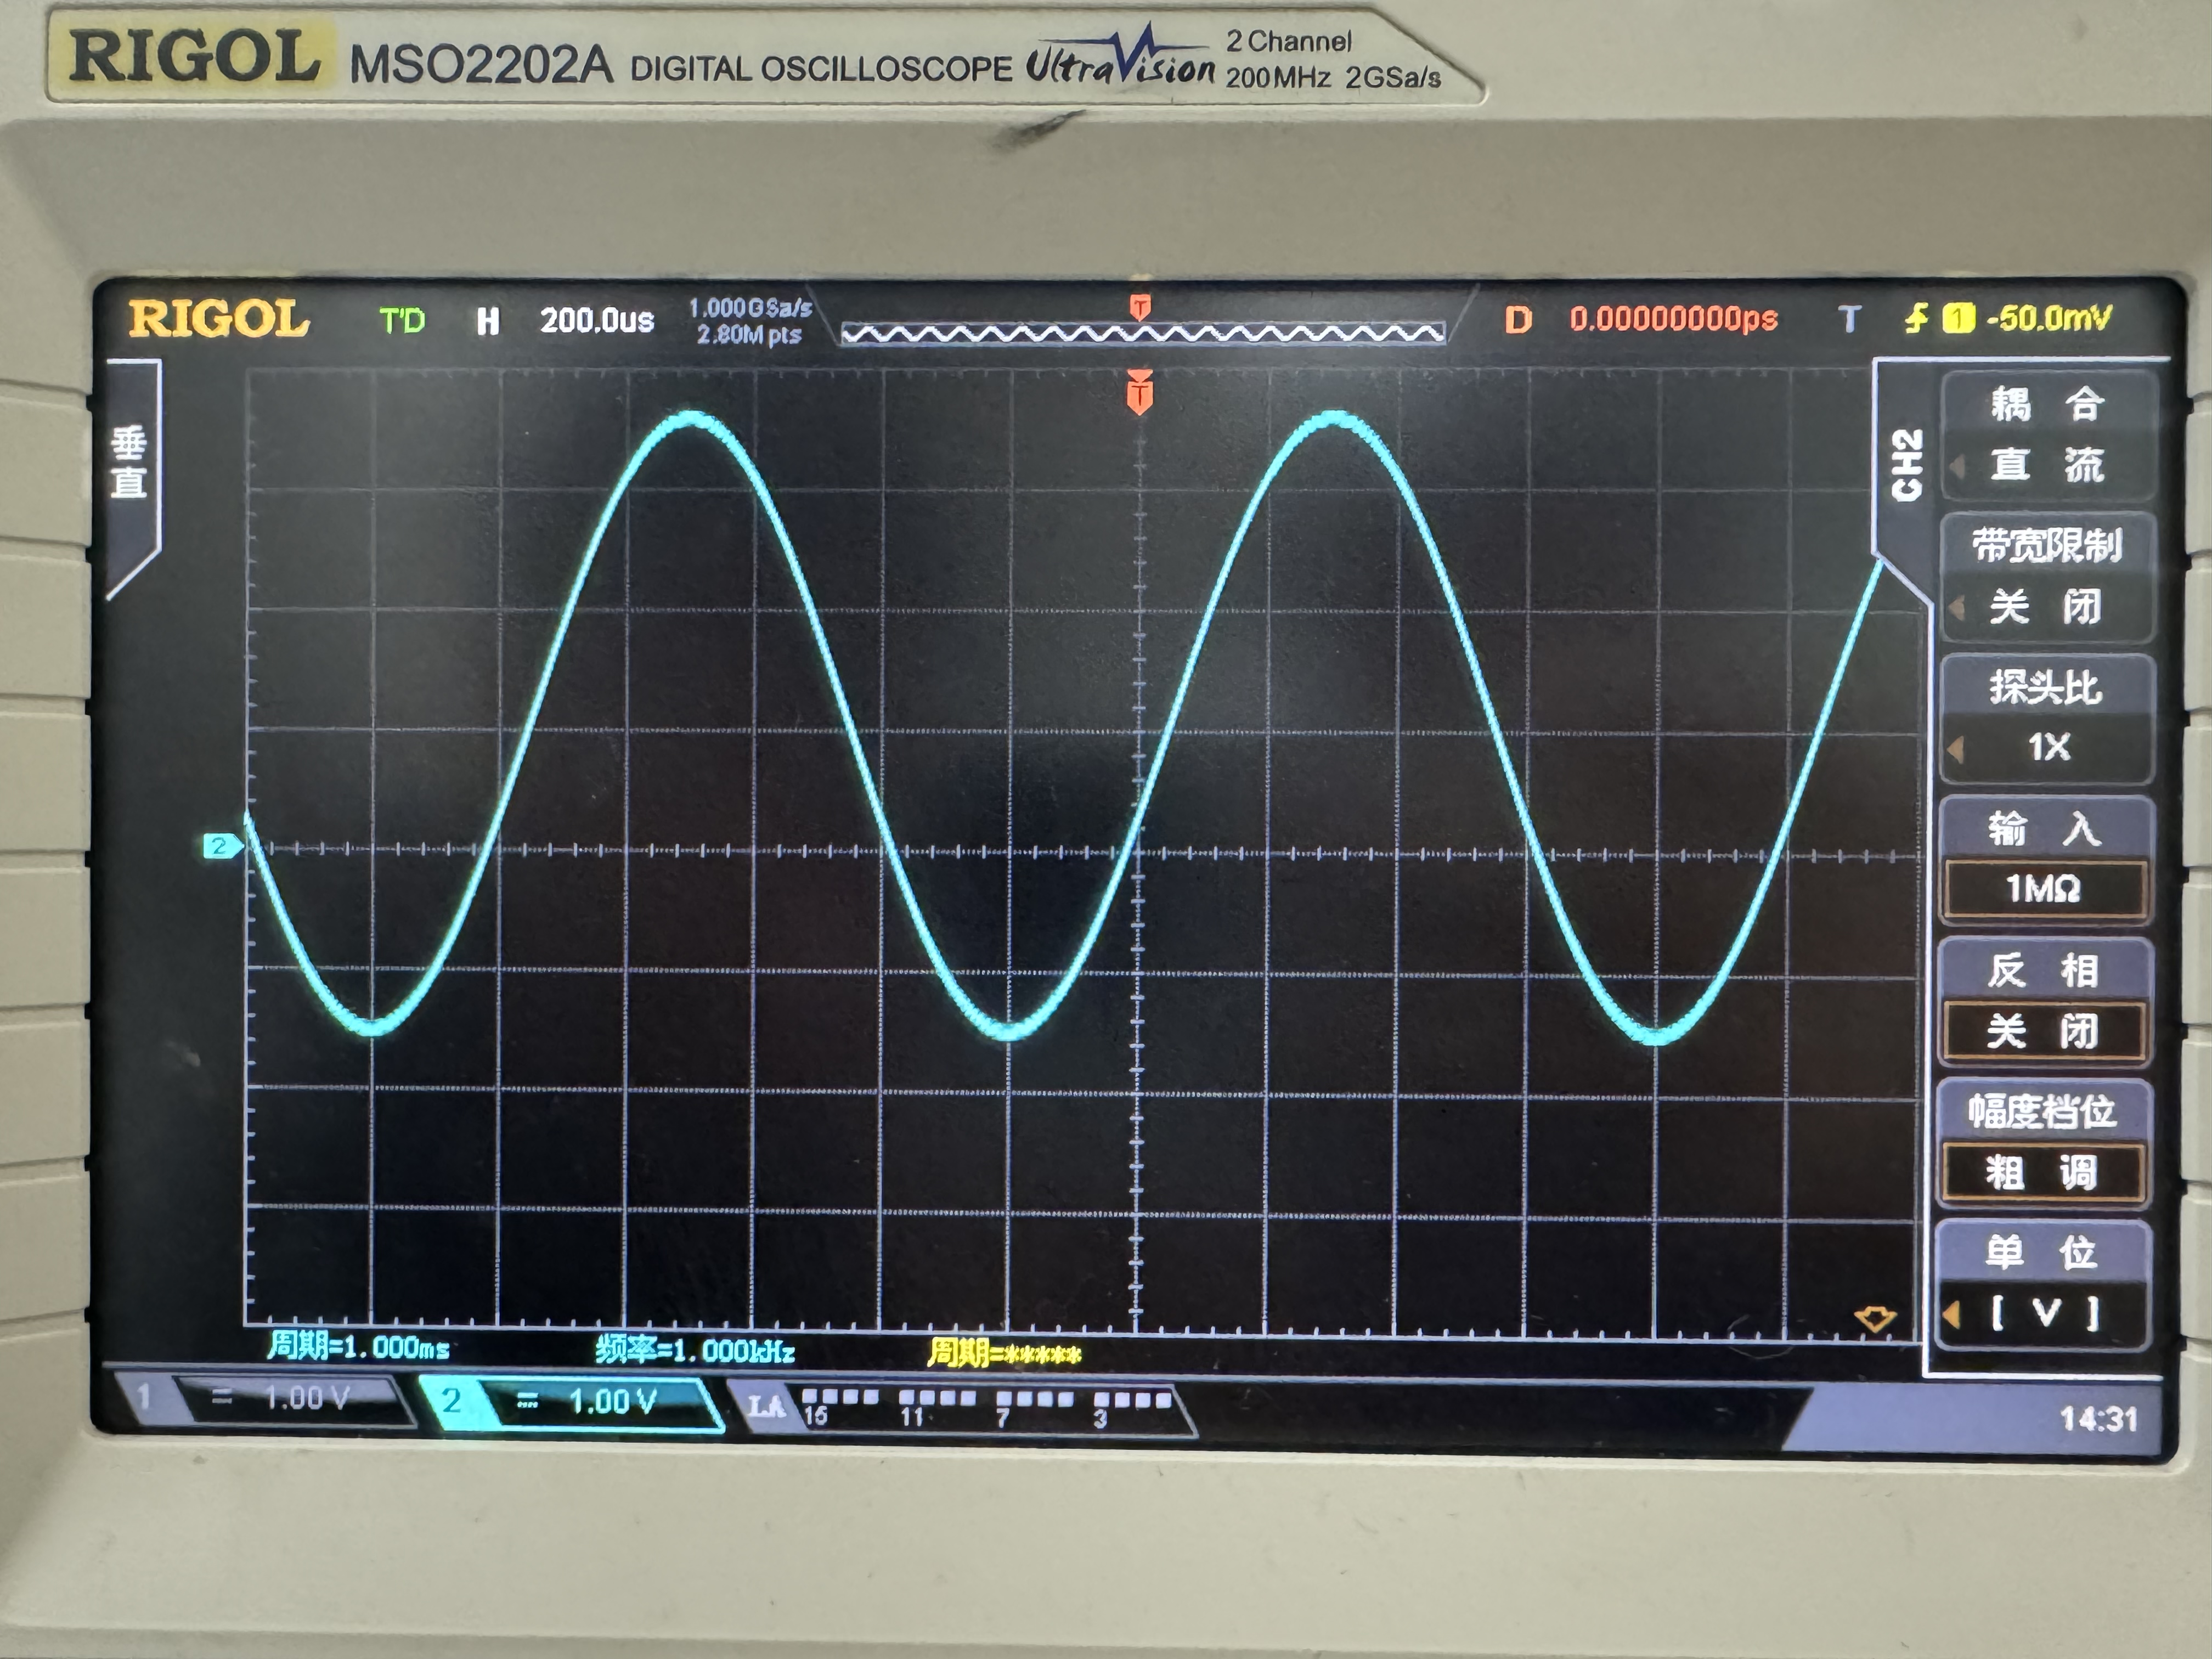
\includegraphics[width=0.4\textwidth]{8_2.jpg}}\hspace{6mm}
    \subfloat[交流耦合\label{fig:8.2b}]{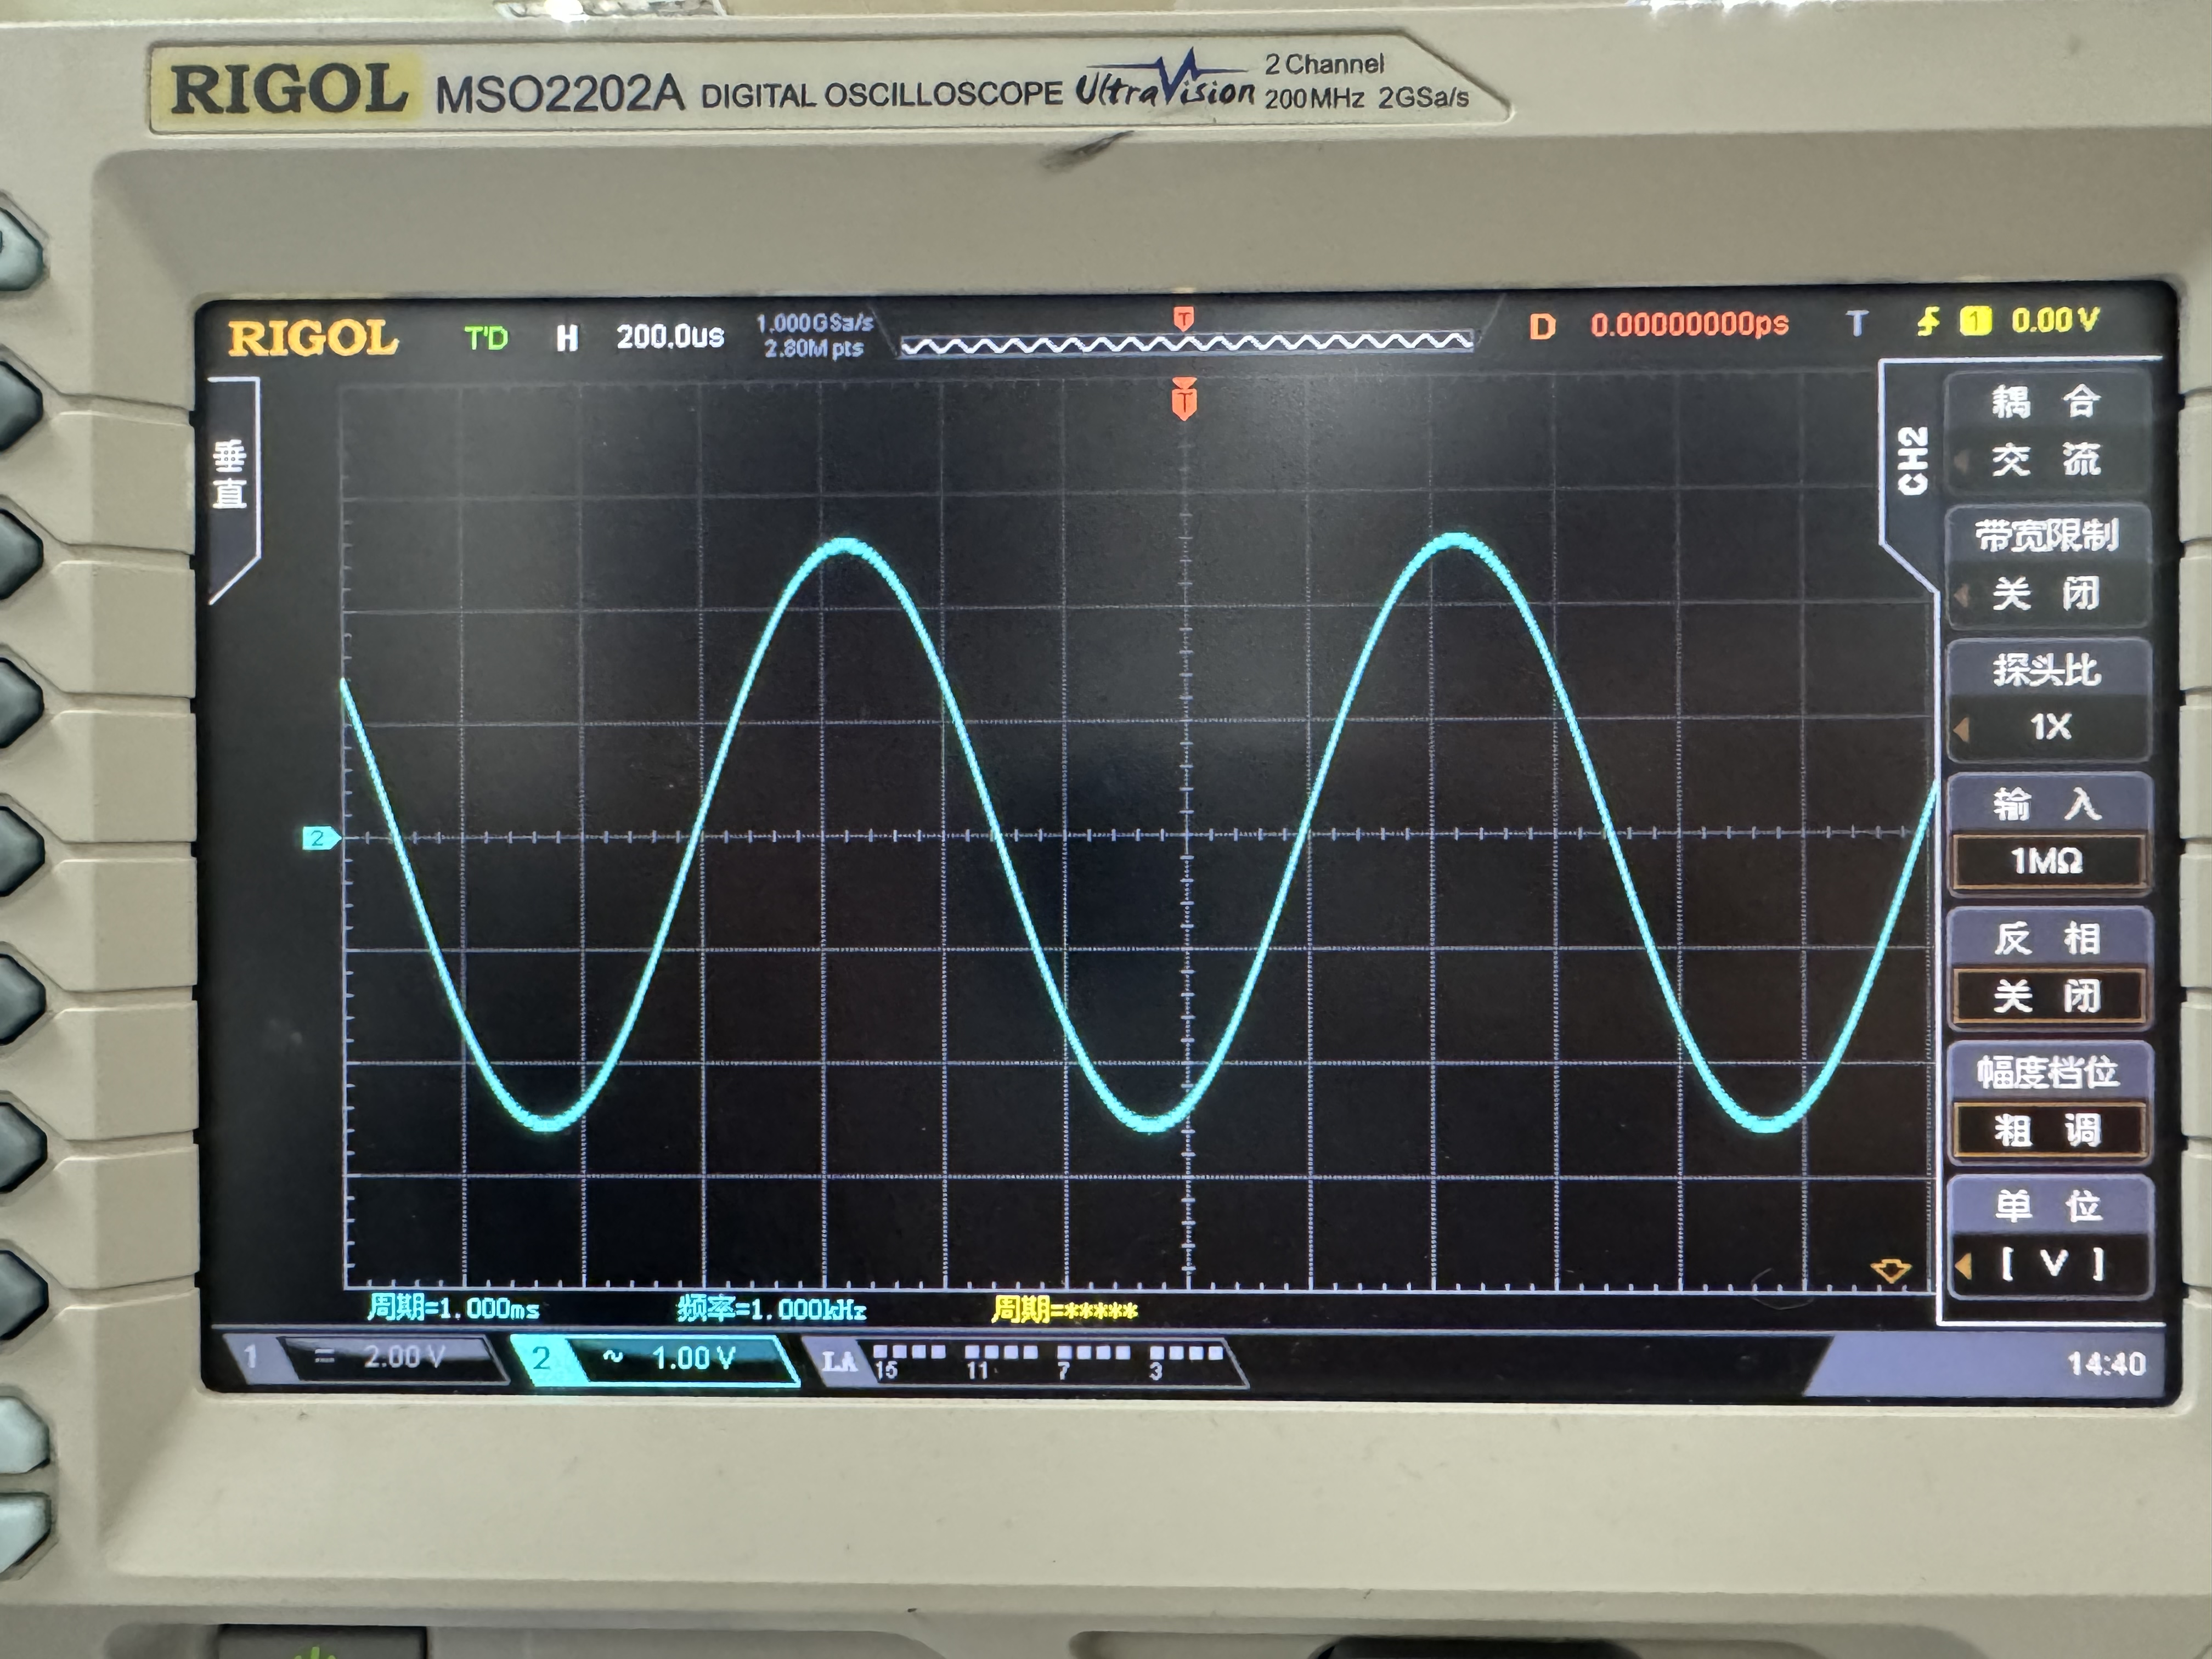
\includegraphics[width=0.4\textwidth]{8_3.jpg}}
    \caption{通道 2 测量偏移为 \SI{1}{\V} 的正弦波\label{fig:8.2}}
\end{figure}

\subsection{观察测量矩形波信号\label{sss:juxingbo}}
设置信号发生器通道 1 输出 $V_\text{pp}=\SI{5}{\V}$,$f=\SI{1}{\kilo\Hz}$,偏移为 \SI{0}{\V},占空比为 50\% 的矩形波,连接到示波器通道 1;设置信号发生器通道 2 输出 $V_\text{pp}=\SI{5}{\V}$,$f=\SI{1}{\kilo\Hz}$,偏移为 \SI{0}{\V},占空比为 20\% 的矩形波,连接到示波器通道 2。调整示波器的水平、垂直和触发等参数,使示波器屏幕上显示 2-3 个完整信号周期,信号幅度占屏幕高度的四分之三左右,波形稳定不移动。测量信号的周期、正占空比、正脉宽等参数并记到表 \ref{tab:8.3},比较两个波形的异同,并保存波形为图 \ref{fig:8.4}。
\begin{table}[!ht]
    \caption{矩形波参数测量\label{tab:8.3}}
    \begin{tabularx}{\textwidth}{|p{5.1em}|X|X|}\hline
        信号发生器设置 & 通道 1 输出 $V_\text{pp}=\SI{5}{\V}$,$f=\SI{1}{\kilo\Hz}$,偏移为 \SI{0}{\V},占空比为 50\% 的矩形波 & 通道 2 输出 $V_\text{pp}=\SI{5}{\V}$,$f=\SI{1}{\kilo\Hz}$,偏移为 \SI{0}{\V},占空比为 20\% 的矩形波 \\ \hline
        & 周期 = \SI{1}{\ms} & 周期 = \SI{1}{\ms} \\
        测量结果 & 正占空比 = 50\% & 正占空比 = 20\% \\
        & 正脉宽 = \SI{500.0}{\us} & 正脉宽 = \SI{200.0}{\us} \\ \hline
    \end{tabularx}
\end{table}
\begin{figure}[!ht]
    \includegraphics[width=0.4\textwidth]{8_4.jpg}
    \caption{矩形波信号\label{fig:8.4}}
\end{figure}

\subsection{观察“同相位”前后的波形并测量相位差\label{sss:tongxiangwei}}
设置信号发生器通道 1、2 均为输出 $V_\text{pp}=\SI{5}{\V}$,$f=\SI{1}{\kilo\Hz}$,偏移为 \SI{0}{\V} 的正弦波,其中通道 1 的初始相位为 $0^\circ$,通道2的初始相位为 $180^\circ$。示波器的两个通道分别与信号发生器的输出连接,两个波形均调到屏幕中间位置(按下垂直 POSITION),使波形稳定不移动,保存波形为图 \ref{fig:8.5}。然后按下信号发生器的“同相位”按键,观察波形的变化并保存波形为图 \ref{fig:8.6}。\par
\begin{figure}[!ht]
    \begin{floatrow}
        \ffigbox{\caption{按下“同相位”前\label{fig:8.5}}}{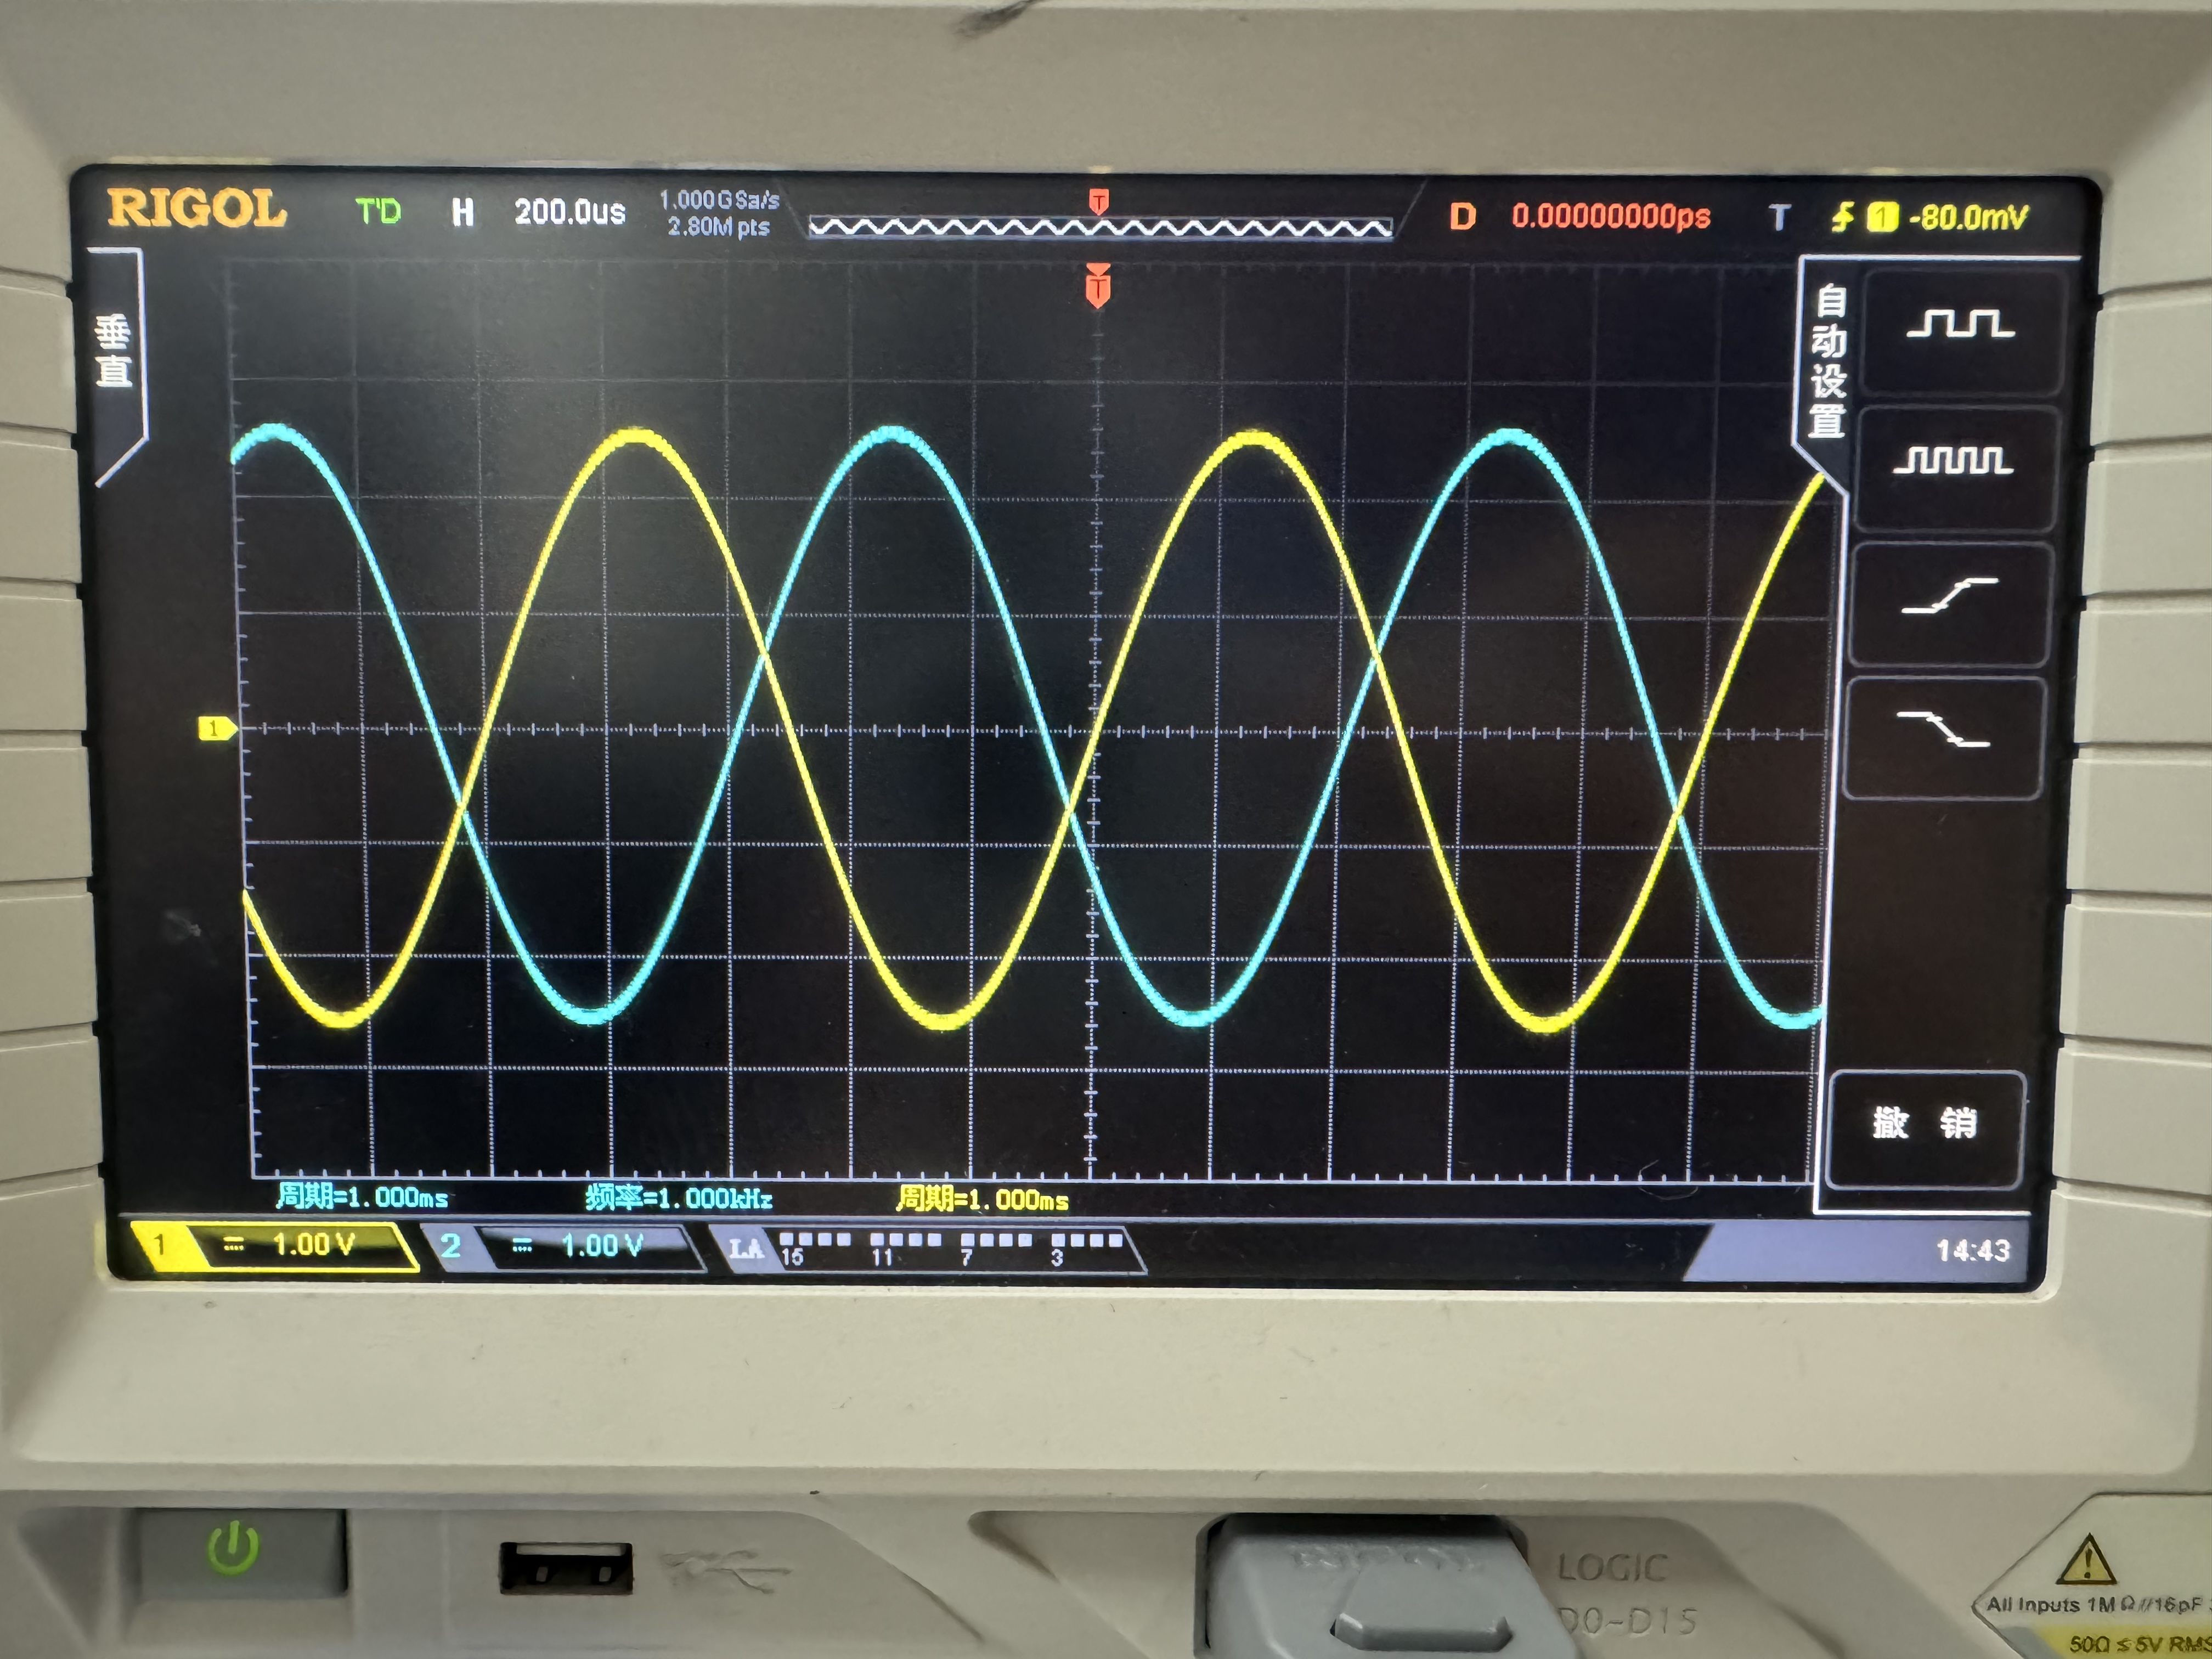
\includegraphics[width=0.4\textwidth]{8_5.jpg}}
        \ffigbox{\caption{按下“同相位”后\label{fig:8.6}}}{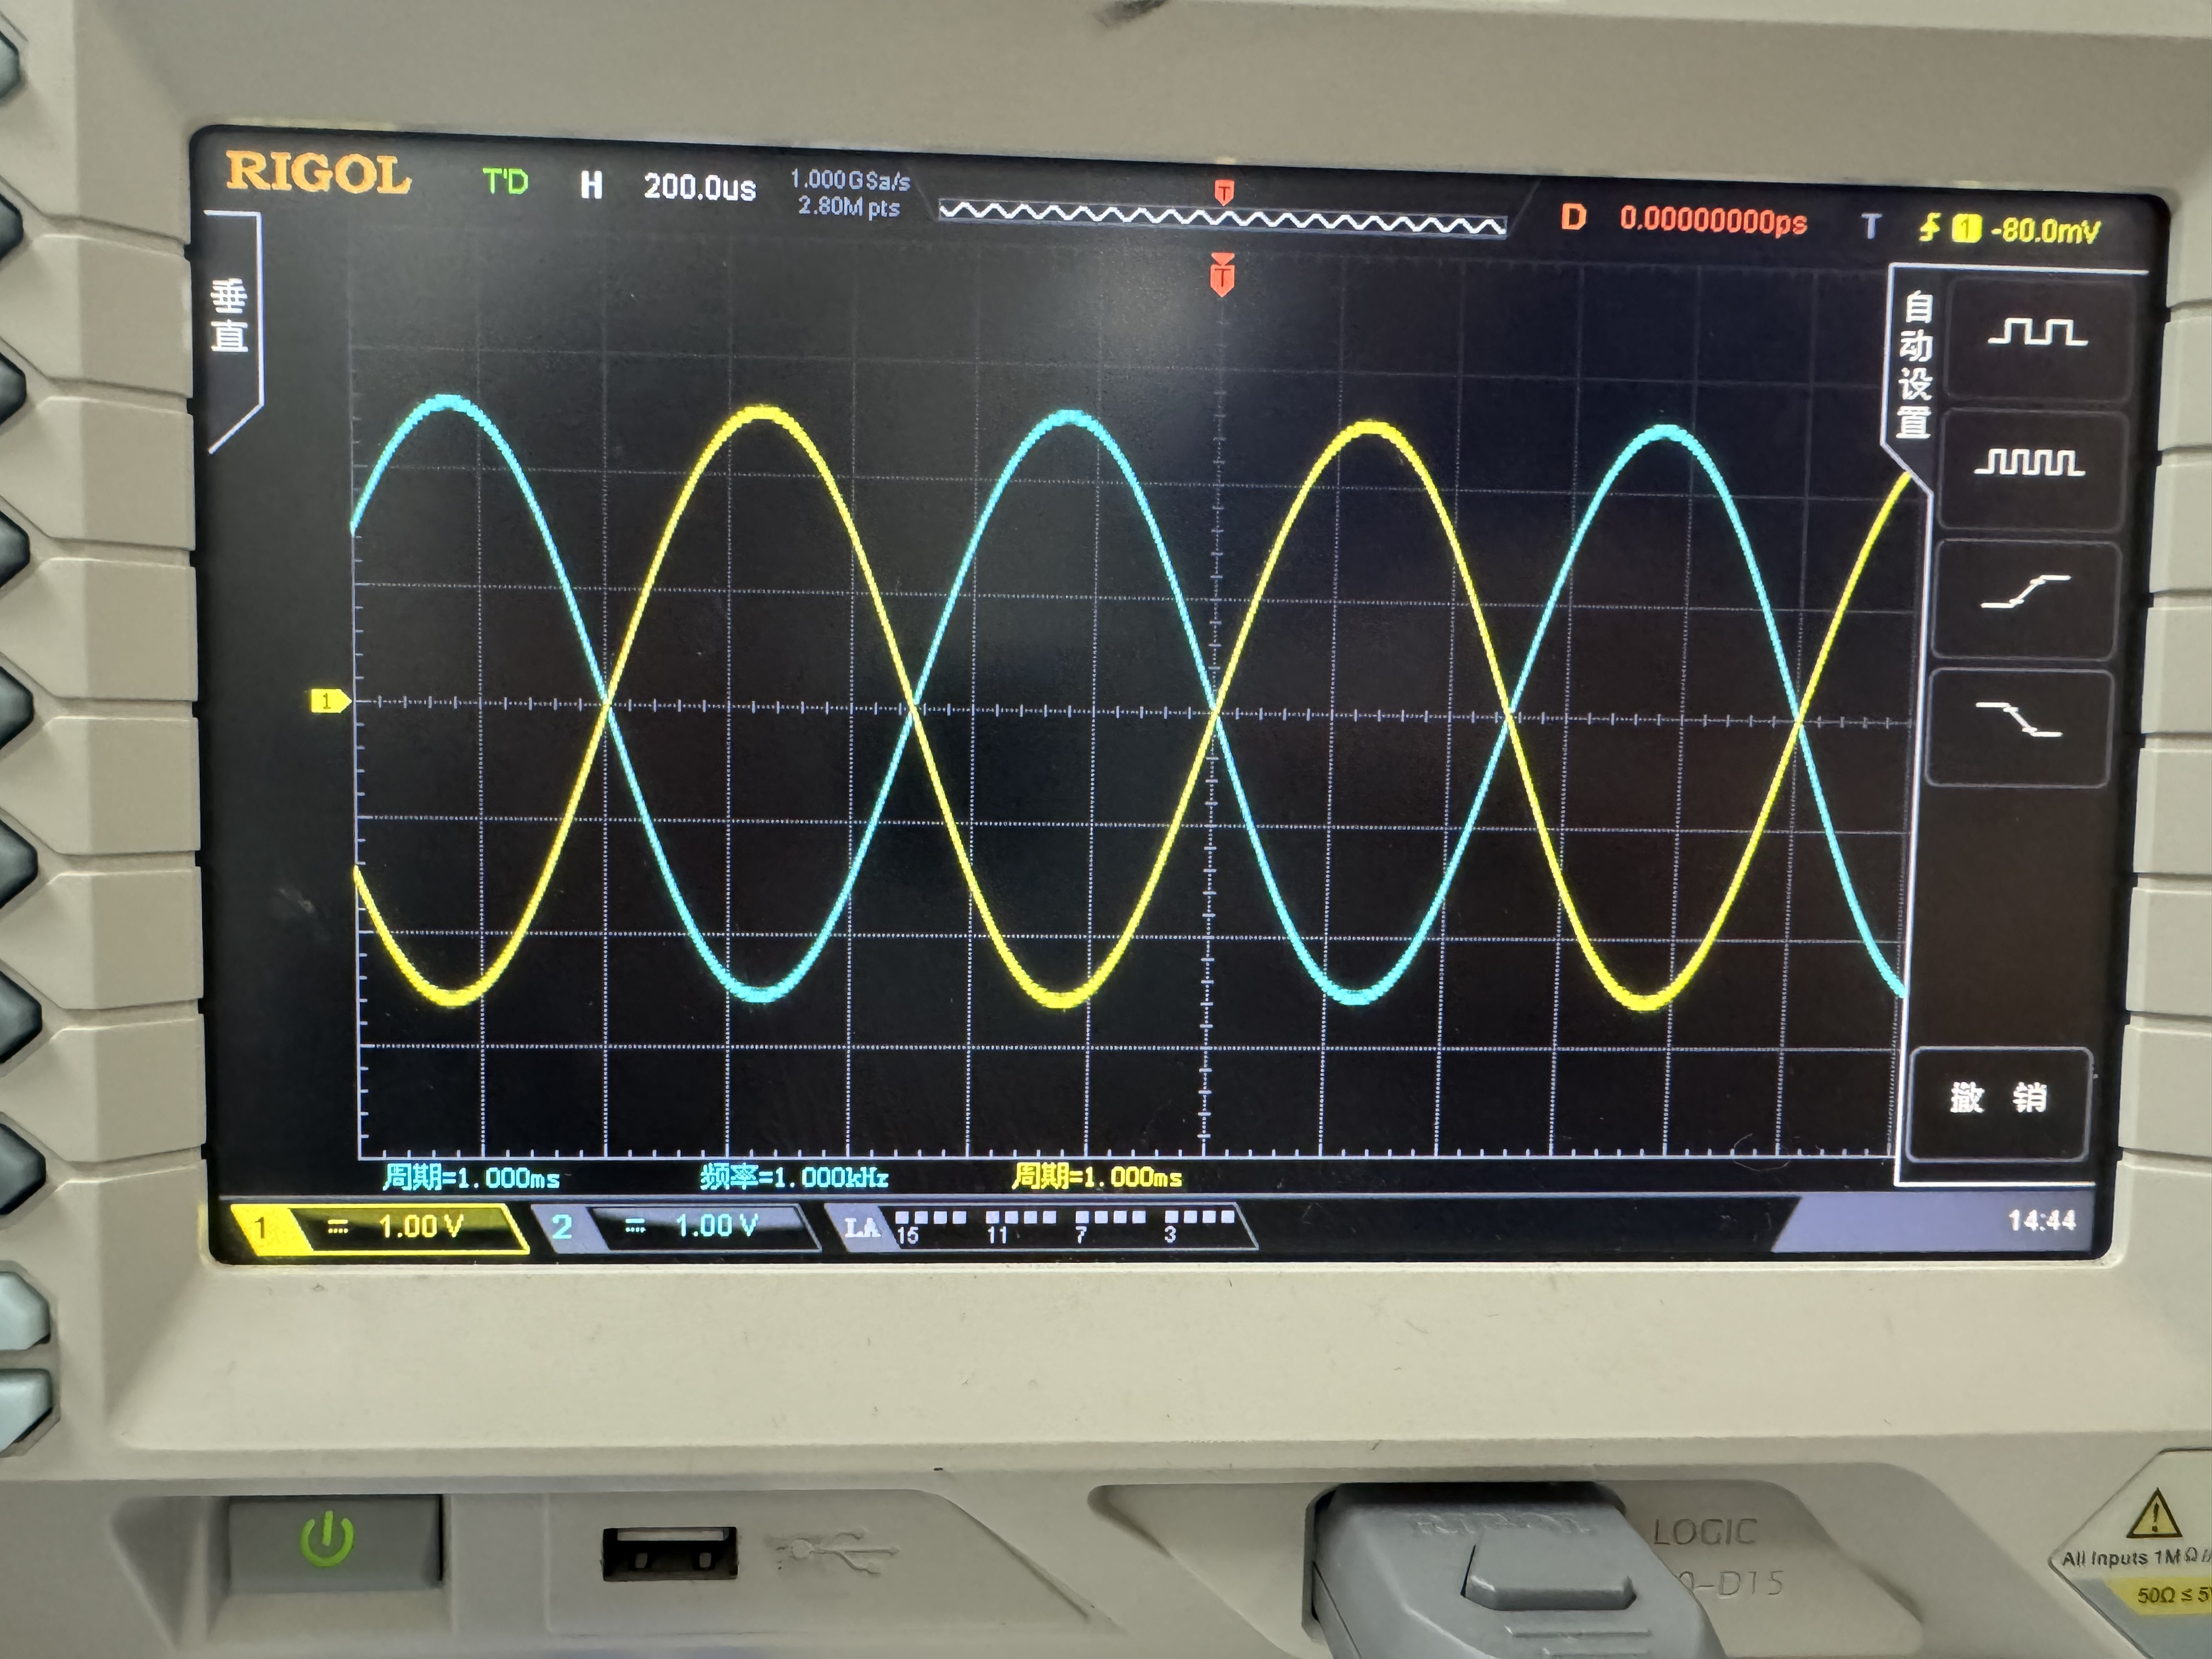
\includegraphics[width=0.4\textwidth]{8_6.jpg}}
    \end{floatrow}
\end{figure}

设置信号发生器通道 1、2 均为输出 $V_\text{pp}=\SI{5}{\V}$,$f=\SI{1}{\kilo\Hz}$,相位差分别为 $45^\circ$ 和 $90^\circ$,使用两种方法测量相位差,结果记录到附表 \ref{tab:8.4}。
\begin{table}[!ht]
    \caption{相位差的测量\label{tab:8.4}}
    \begin{tabularx}{\textwidth}{|*{3}{C|}}\hline
        信号相位差 & 光标测量法 & 自动测量法 \bigstrut \\ \hline
        $45^\circ$ & $-44.64^\circ$ & $-44.64^\circ$ \bigstrut \\ \hline
        $90^\circ$ & $-88.50^\circ$ & $-90.72^\circ$ \bigstrut \\ \hline
    \end{tabularx}
\end{table}

\subsection{观察李沙育(Lissajous,也有译为李萨如)波形}
将两个同频率、同幅度的正弦信号分别加到示波器的 X 轴和 Y 轴,当两个信号的相位差为 $0^\circ$ 时,李沙育图形是一条跟 X 轴成 $45^\circ$ 的直线;当两个信号的相位差为 $45^\circ$ 时,李沙育图形是一个椭圆;当两个信号的相位差为 $90^\circ$ 时,李沙育图形是一个圆。\par
改变示波器水平控制时基选项,从 Y-T 调整为 X-Y,设置信号发生器通道 1、2 均为输出 $V_\text{pp}=\SI{5}{\V}$,$f=\SI{1}{\kilo\Hz}$,偏移为 \SI{0}{\V} 的正弦波,相位差分别为 $0^\circ$、$45^\circ$、$90^\circ$,按下“同相位”按键,观察并记录李沙育波形,分别保存波形为图 \ref{fig:8.7}、图 \ref{fig:8.8}、图 \ref{fig:8.9}。
\begin{figure}[!ht]
    \begin{floatrow}[2]
        \ffigbox{\caption{相位差 $0^\circ$\label{fig:8.7}}}{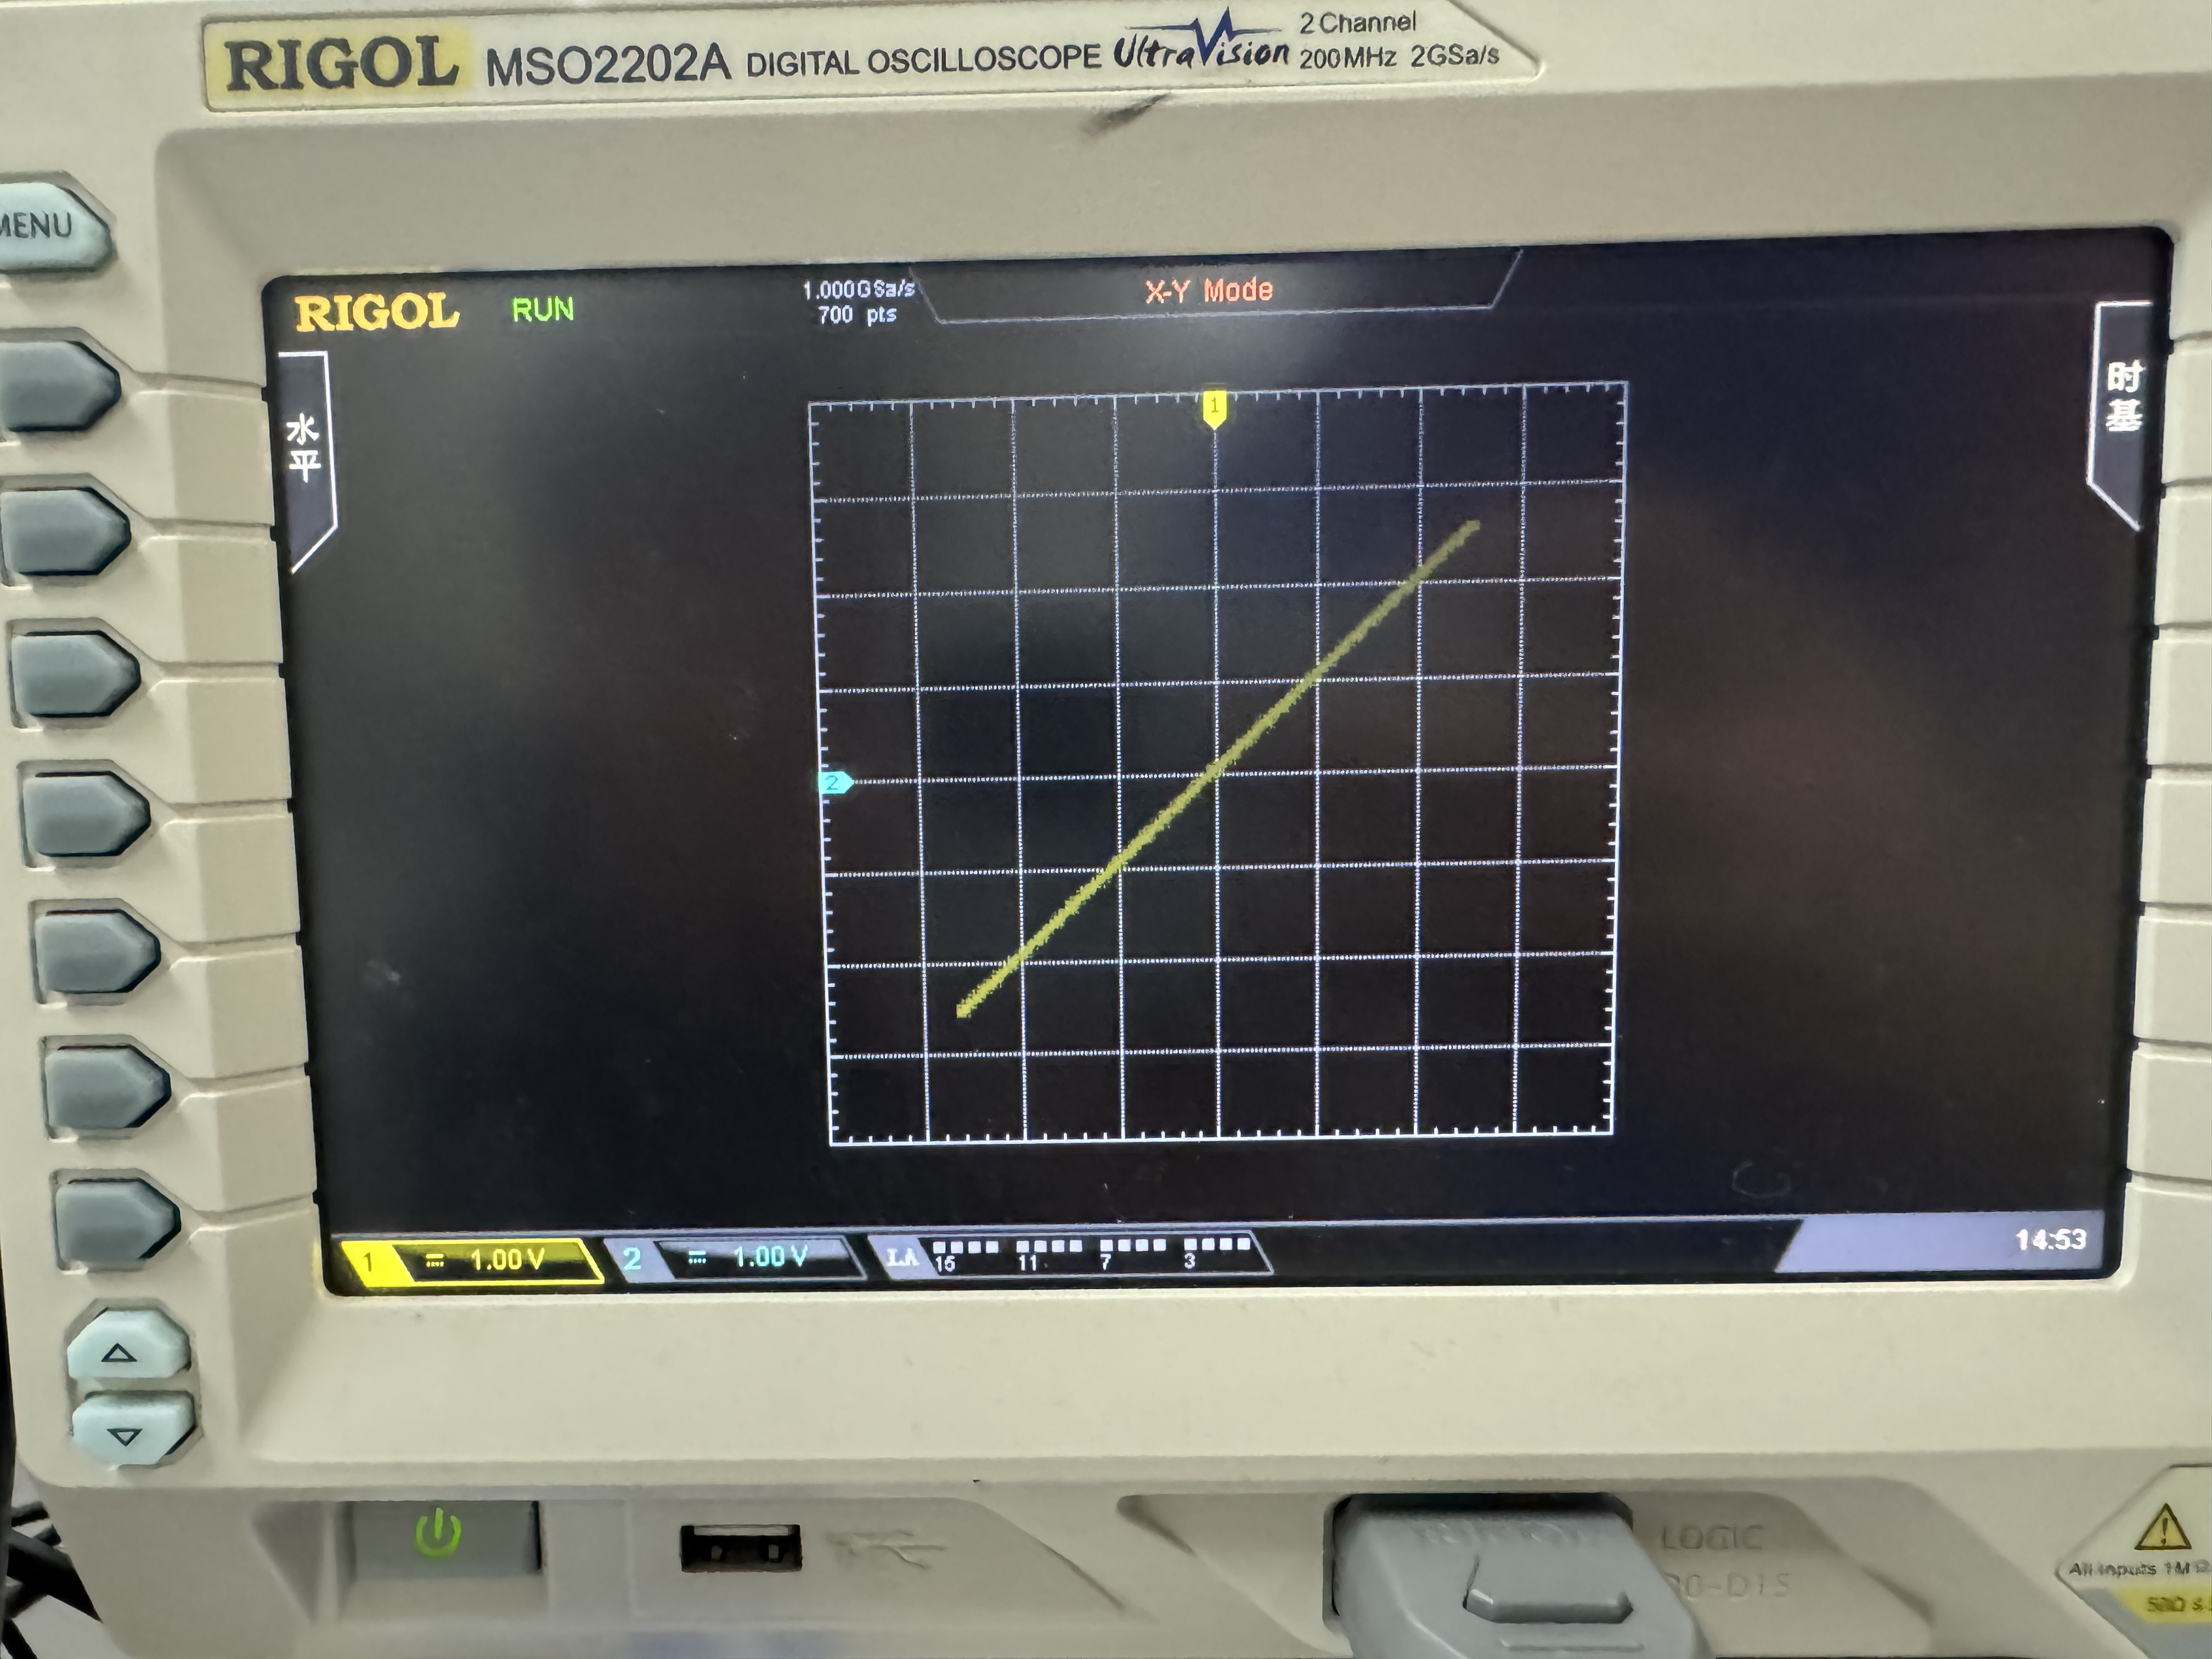
\includegraphics[width=0.4\textwidth]{8_9.jpg}}
        \ffigbox{\caption{相位差 $45^\circ$\label{fig:8.8}}}{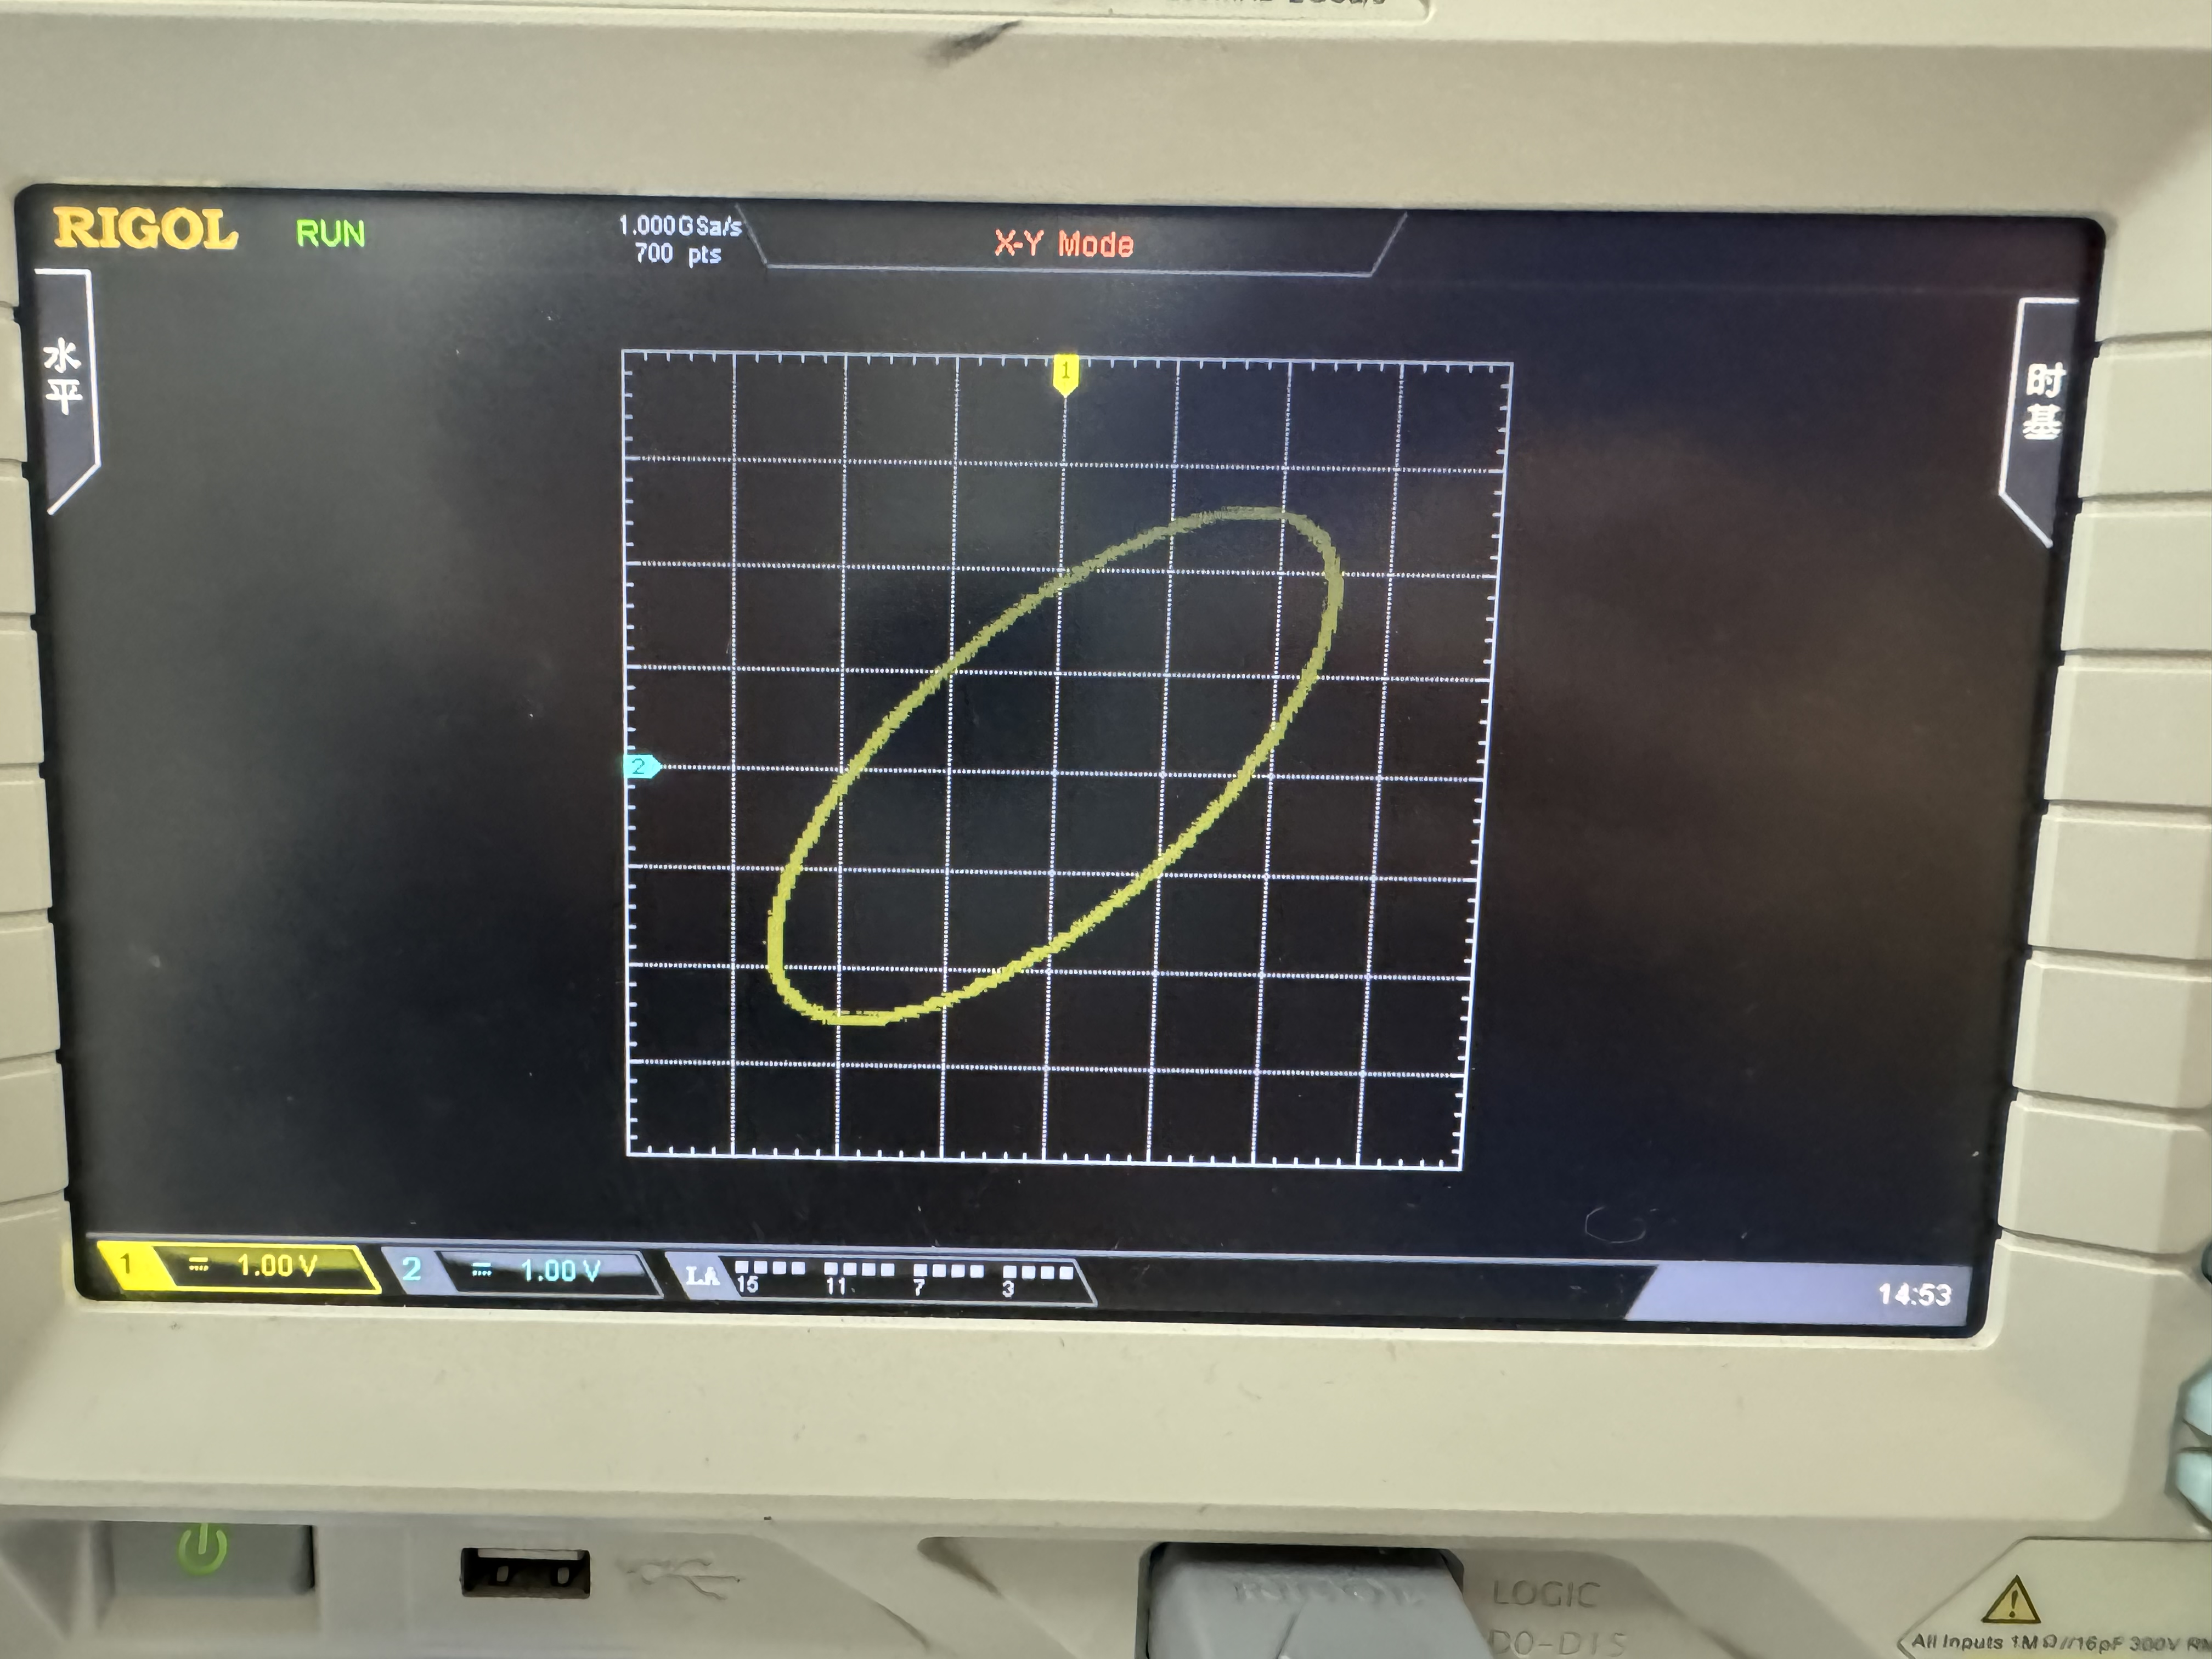
\includegraphics[width=0.4\textwidth]{8_8.jpg}}
    \end{floatrow}
\end{figure}
\begin{figure}[!ht]
    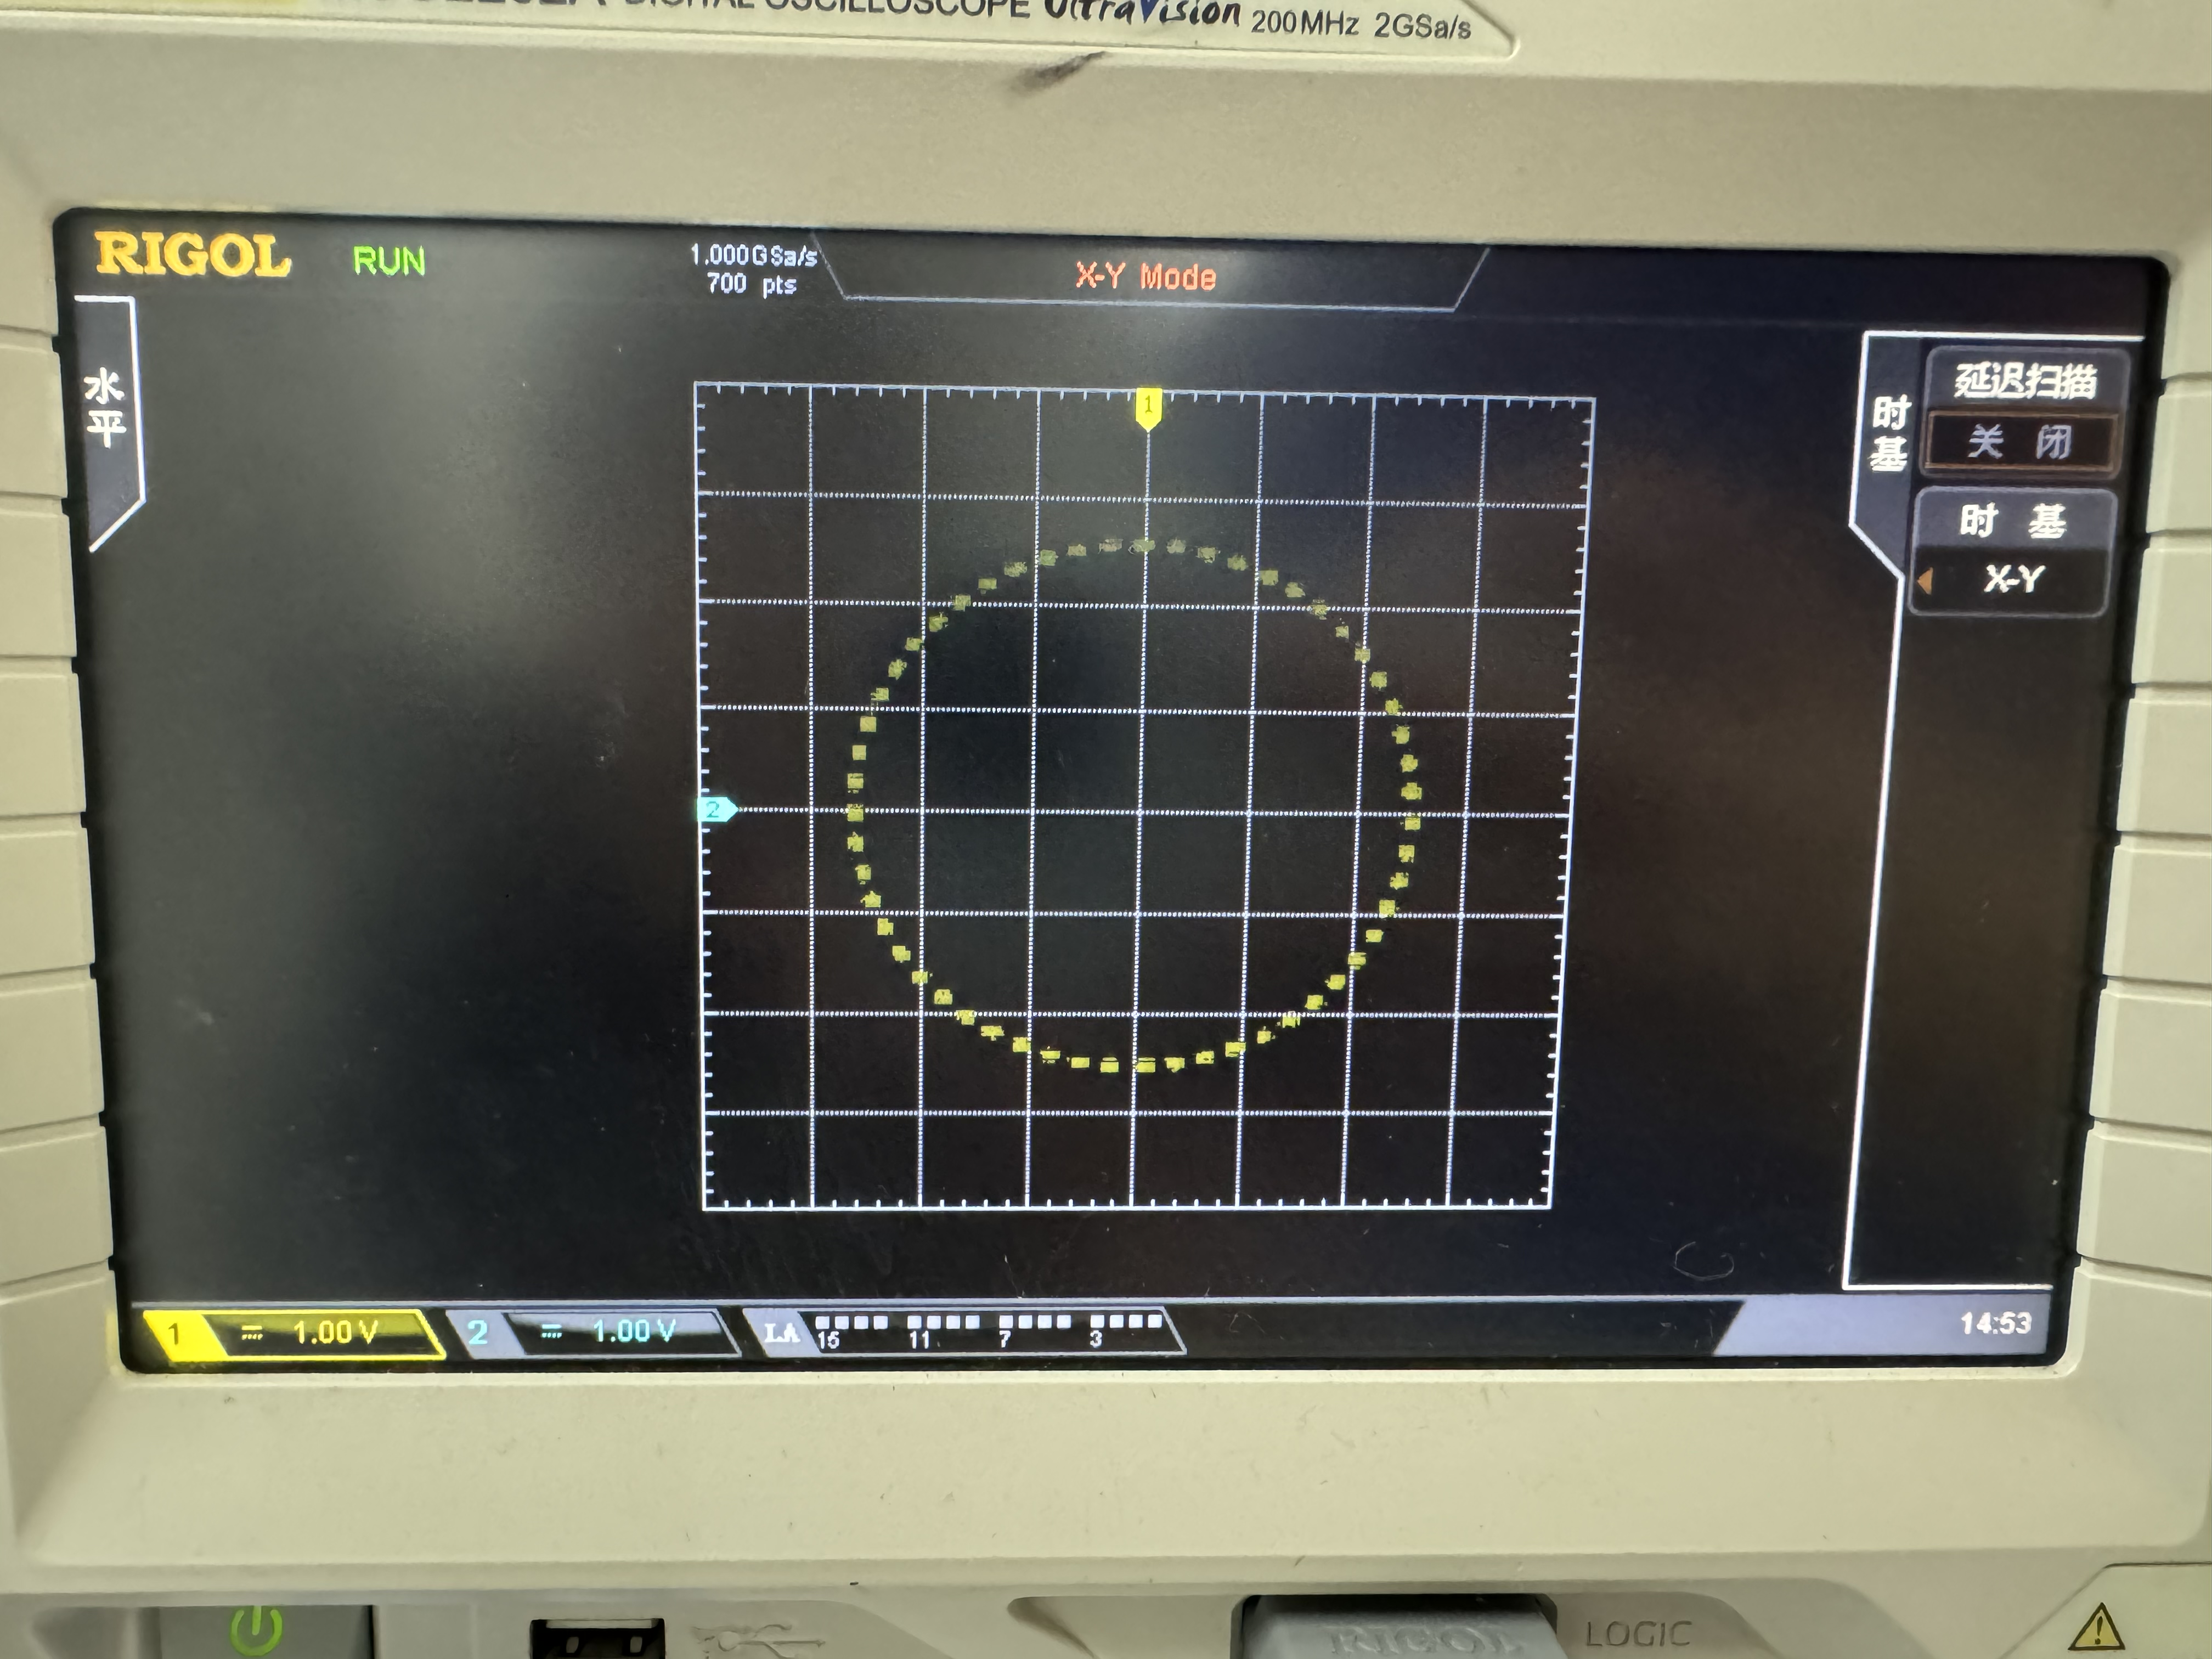
\includegraphics[width=0.4\textwidth]{8_7.jpg}
    \caption{相位差 $90^\circ$\label{fig:8.9}}
\end{figure}
\section{实验分析}

\subsection{分析}
实验 \Nameref{sss:ouhe}时,直流耦合的波形位置有偏移,能看到偏移量,而交流耦合没办法看到偏移量。实验 \Nameref{sss:juxingbo}时,占空比 50\% 的矩形波比占空比 20\% 的矩形波要宽很多。实验 \Nameref{sss:tongxiangwei}时,按下同相位前波形没有完全对上,按下同相位后,波形就完全对上了。
\subsection{误差分析}
    \begin{enumerate}
        \item 万用表在测量电阻时会有内部电阻,这个电阻值会对测量结果产生影响,特别是在测量较小阻值时。
        \item 选择不当的测量范围也可能导致误差,如果选择的范围过大,测量会不准确;如果选择的范围过小,则可能会损坏仪器或导致不准确的读数。此次实验量程为自动确定,不能确定是是否选到了合适的量程。
        \item 温度、湿度等环境因素也会对测量结果产生影响。
        \item 元件长时间摆放导致内部结构发生变化,导致实际值发生变化。
        \item 示波器接入原电路后会对原电路的结构有一定影响,导致测量结果不准确。
    \end{enumerate}
\section{实验心得}
此次实验测量了常用电信号。在实际操作中,观察到了由于仪器误差和连接线电阻带来的微小偏差,但总体上实验结果符合理论预期。这些实验提升了我使用示波器的技能。
\clearpage
\section{原始数据}
\begin{center}
    \framebox{\rotatebox{-90}{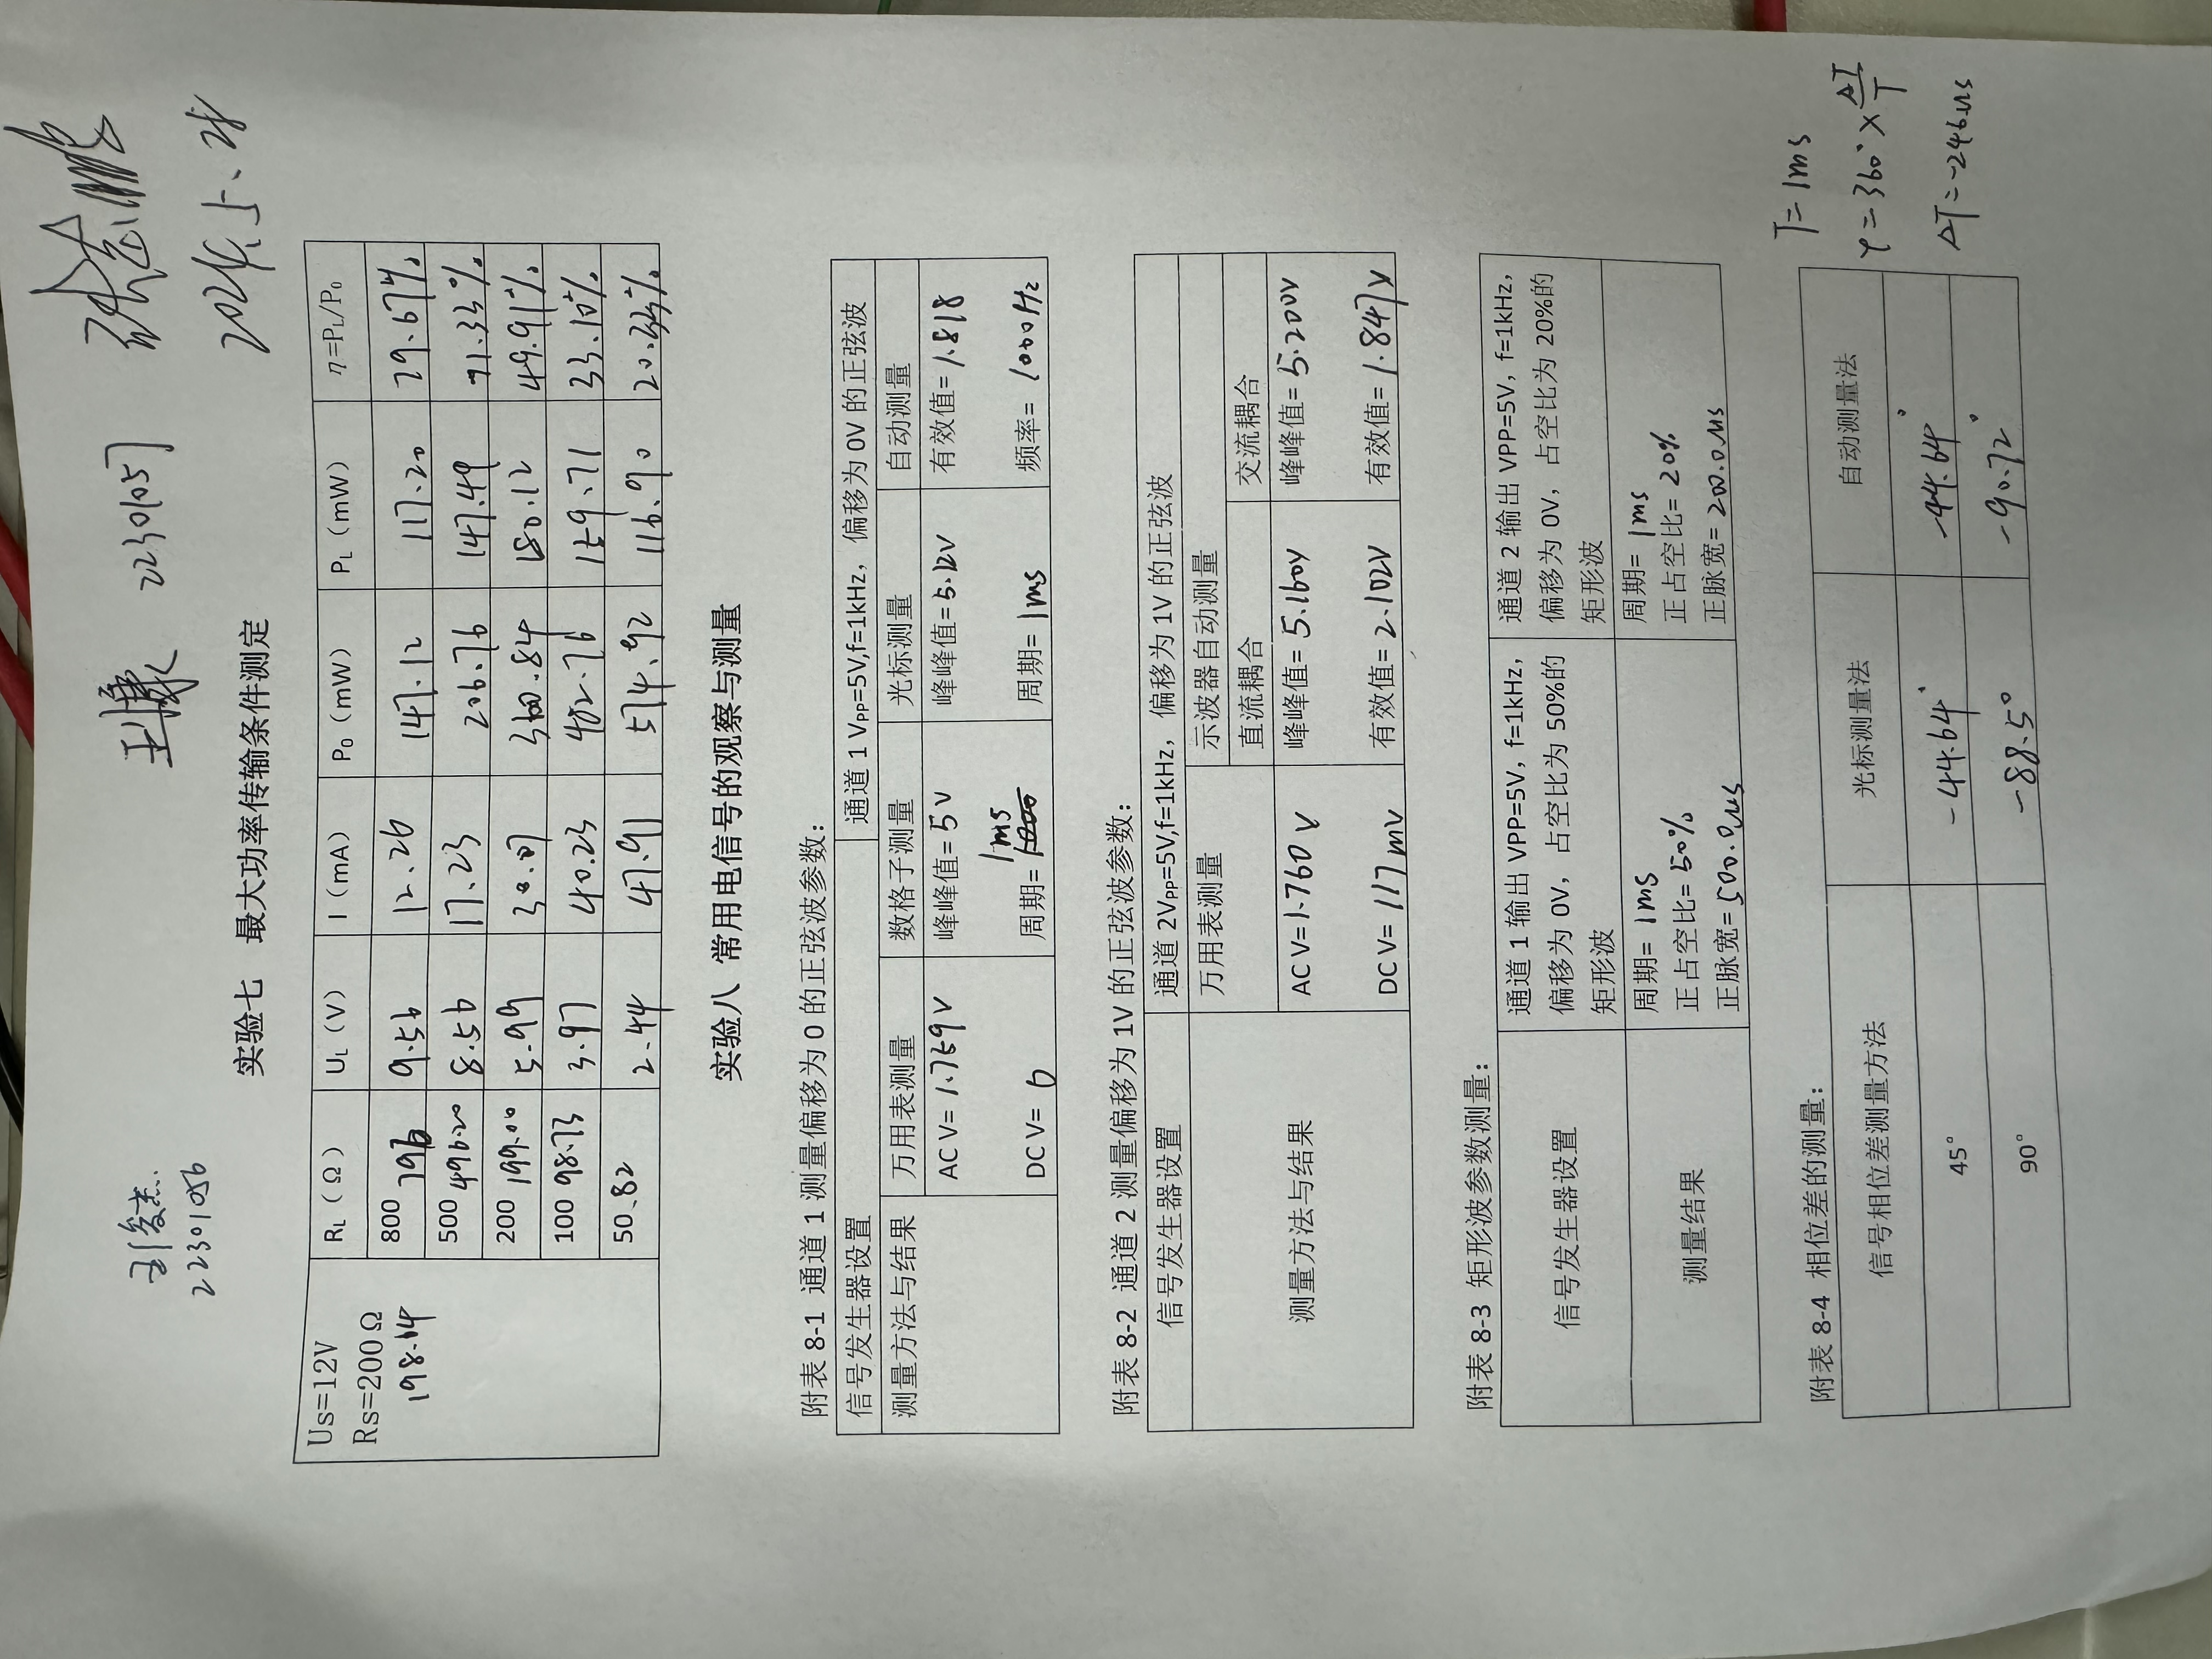
\includegraphics[height=0.95\textwidth]{rawdata.jpg}}}
\end{center}
\end{document}